\chapter{有理数}

\section{有理数的意义}\label{sec:1-1}

\subsection{正数和负数}\label{subsec:1-1}

我们在生产劳动和日常生活中需要计算物体的个数,就使用了自然数 1、2、3、……;
为了用数表示没有物体,就使用了数 0 ;
在测量物体的长度、重量等的时候,往往不能正好得到整数的结果,就使用了分数和小数。
这些数我们在小学已经学习过了。

只有这些数能不能满足实际需要呢?我们看下面的例子:
有一天最高温度是零上 5 ℃(℃ 读作摄氏度),最低温度是零下 5 ℃(图 \ref{fig:1-1})。
要表示出这两个温度,如果只用小学学过的数,把它们都记作 5 ℃,就不能把它们区别清楚。

\begin{figure}[htbp]
    \centering
    \begin{minipage}{7cm}
    \centering
    \begin{tikzpicture}
    \draw (0,0) pic {thermometer={5}};
    \draw (3,0) pic {thermometer={-5}};
\end{tikzpicture}

    \caption{}\label{fig:1-1}
    \end{minipage}
    \qquad
    \begin{minipage}{7cm}
    \centering
    \begin{tikzpicture}[>=Stealth, scale=1.5]
    \draw [rounded corners=6pt, ground]
        (0, 0) .. controls (1,0) and (1,0) .. (1.5,3)
            -- (3, 3) .. controls (3,2) and (3,1) .. (4, 0.2);
    \draw [<->] (0.5, 0.05) -- (0.5, 1.2)
        node[pos=.5, rotate=90, fill=white, inner sep=0] {\small 3.6}
        node[pos=-0.05, fill=white, inner sep=1pt, below] {\small 乙};
    \draw [dashed] (0.2, 1.2) -- (4, 1.2);
    \draw [<->] (3.8, 1.2) -- (3.8, 3)
        node[pos=.5, rotate=90, fill=white, inner sep=0] {\small 5.2};
    \node at (3, 3) [fill=white, inner sep=1pt, anchor=south east] {\small 甲};
    \draw [dashed] (3, 3) -- (4.5, 3);
    \draw (4.1, 1.4) -- (4.3, 1.4) -- (4.2, 1.2) -- cycle;
    \path [path picture={\draw (path picture bounding box.north west) pic {waterwave};}] (3.2, 1.2) -- (4.5, 1.2) -- (3.9, 0.6) -- cycle;
\end{tikzpicture}

    \caption{}\label{fig:1-2}
    \end{minipage}
\end{figure}

零上 5 ℃ 和零下 5 ℃ 虽然都是 5 ℃,但是它们的意义是相反的,
一个在 0 ℃ 的上面, 一个在 0 ℃ 的下面。
为了区别这种具有相反意义的量,我们把零上 5 ℃ 记作 $+5$ ℃ (读作正 5 摄氏度)或 5 ℃;
把零下 5 ℃ 记作 $-5$ ℃(读作负 5 摄氏度)。
也就是说,我们把一种意义的量——零上温度规定为正的,把另一种与它相反意义的量——零下温度规定为负的。
正的量用小学学过的数的前面放上 “$+$”(读作正)号来表示,也可以把 “$+$” 号省略不写,仍旧用以前学过的数表示;
负的量就用小学学过的数的前而放上“$-$” (读作负)号来表示。

\begin{enhancedline}
具有相反意义的量的例子很多,例如,甲地高出海平面 5.2 米,乙地低于海平面 3.6 米(图 \ref{fig:1-2});
昨天运进货物 $8\dfrac{1}{2}$ 吨, 今天运出货物 $4\dfrac{1}{2}$ 吨; 等等。
我们可以把高出海平面 5.2 米记作 $+5.2$ 米或 5.2 米,低于海平面 3.6 米记作 $-3.6$ 米;
运进货物 $8\dfrac{1}{2}$ 吨记作 $+8\dfrac{1}{2}$ 吨 或 $8\dfrac{1}{2}$,
运出货物 $4\dfrac{1}{2}$ 吨记作  $-4\dfrac{1}{2}$ 吨。
\end{enhancedline}


\lianxi
1.(口答) 举出一些具有相反意义的量的实例。

2.(口答) 如果向东走 5 千米记作 $+5$ 千米,那么向西走 6 千米记作什么?

3.(口答) 如果下降 400 米记作 $-400$ 米,那么上升 800 米记作什么?

4.(口答) 如果节余 10.32 元记作 $+10.32$ 元,那么亏损 4.15 元记作什么?

\jiange

\begin{enhancedline}
象 $+5$、$+8\dfrac{1}{2}$、$+5.2$ 等带有正号的数叫做\zhongdian{正数}(正号也可省略不写)。
象 $-5$、$-4\dfrac{1}{2}$、$-3.6$ 等带有负号的数叫做\zhongdian{负数}。
零既不是正数, 也不是负数。
\end{enhancedline}

\lianxi
(口答)读出下列各数,它们各是正还是负数?

\begin{enhancedline}
$+6$,$-8.75$,$-0.4$,$0$,$\dfrac{3}{7}$,$9.15$,$-\dfrac{2}{3}$,$+1\dfrac{4}{5}$。

\jiange

\liti[0] 所有的正数组成正数集合,所有的负数组成负数集合。
把下列各数中的正数和负数分别填在表示正数集合和负数集合的圈里:

$-11$,$4.8$,$+73$,$-2.7$,$\dfrac{1}{6}$,$+\dfrac{7}{12}$,$-8.12$,$-\dfrac{3}{4}$。
\end{enhancedline}

\begin{figure}[htbp]
    \centering
    \begin{tikzpicture}
    \draw (2, 0) circle [x radius=2, y radius=1];
    \node at (2, -1.5) {正数集合};
    \draw (8,0) circle [x radius=2, y radius=1];
    \node at (8, -1.5) {负数集合};
\end{tikzpicture}

    \caption{}\label{fig:1-3}
\end{figure}

\jie
\begin{figure}[htbp]
    \centering
    \begin{tikzpicture}
    \draw (2, 0) circle [x radius=2, y radius=1];
    \node at (2, -1.5) {正数集合};
    \draw (8,0) circle [x radius=2, y radius=1];
    \node at (8, -1.5) {负数集合};

    \node at (0.8, 0.5) {$4.8$};
    \node at (1.8, 0.5) {$+73$};
    \node at (2.8, 0.5) {\Large $\frac{1}{6}$};
    \node at (1.8, -0.5) {\Large $+\frac{7}{12}$};
    \node at (2.8, -0.5) {……};

    \node at (7.0, 0.5) {$-11$};
    \node at (8.0, 0.5) {$-2.7$};
    \node at (6.9, -0.5) {$-8.12$};
    \node at (7.9, -0.5) {\Large $-\frac{3}{4}$};
    \node at (8.9, -0.5) {……};
\end{tikzpicture}

    \caption{}\label{fig:1-4}
\end{figure}

到现在为止,我们学过的数有:

正整数(也叫自然数),如 $+1$ 、$+2$ 、$+3$、……;

零, $0$;

负整数,如 $-1$ 、$-2$ 、$-3$、……;

\begin{enhancedline}
正分数,如 $+8\dfrac{1}{2}$、 $+5.2 \; \left( \text{即} +5\dfrac{1}{5} \right)$ 、$\dfrac{2}{3}$、……;

负分数,如 $-4\dfrac{1}{2}$、 $-3.6 \; \left( \text{即} -3\dfrac{3}{5} \right)$ 、$-\dfrac{6}{7}$、……;

正整数、零、负整数统称\zhongdian{整数},正分数、负分数统称\zhongdian{分数}。
\end{enhancedline}

整数和分数统称\zhongdian{有理数}。

\zhuyi 整数也可看作是分母为 1 的分数,因此分数包括整数。
有时为了研究需要,也把整数和分数分开,这里的分数是指不包括整数的分数。


\lianxi
\begin{xiaotis}
\begin{enhancedline}
\xiaoti{(口答)下列各数,是整数还是分数,是正数还是负数?\\
    $-7$, $10.1$, $-\dfrac{1}{6}$, $89$, $0$, $-0.67$, $1\dfrac{3}{5}$。
}

\xiaoti{(口答)说出几个正整数、负整数、正分数、负分数。}
\end{enhancedline}
\end{xiaotis}


\subsection{数轴}\label{subsec:1-2}

生活中,常常在一条直线上画出刻度,用这些刻度来表示量的大小。
例如,利用温度计上的刻度来表示温度的高低:零上一个刻度,表示 1 ℃;零下两个刻度,表示 $-2$ ℃;……。
又如,用直尺上的刻度表示长度的大小,用秤杆上的金星表示重量的大小,等等。

同样,我们可以在一条直线上画出点,用这些点表示正数和负数,方法如下。

如图 \ref{fig:1-5},画一条直线(一般画水平的直线),在这条直线上任取一点 $O$ 作为\zhongdian{原点},用这点表示零。
规定这条直线的一个方向为正方向(一般取从左到右的方向),那么相反的方向就是负方向。
再任意取一条线段的长度作为单位长度。

\begin{figure}[htbp]
    \centering
    \begin{tikzpicture}[>=Stealth]
    \draw [->] (-7,0) -- (7.2,0);
    \foreach \x in {-7,...,+6} {
        \draw (\x,0.4) -- (\x,0);
        \foreach \tmp in {1,...,9} {
            \draw (\x+\tmp/10, 0.2) -- (\x+\tmp/10, 0);
        }
        \draw (\x+0.5, 0.3) -- (\x+0.5, 0);
    }

    \foreach \x in {-6,...,0} {
        \node at (\x, -0.3) {$\x$};
    }

    \foreach \x in {1,...,6} {
        \node at (\x, -0.3) {$+\x$};
    }


    \foreach \pos/\text in {-4/B, -1.5/D, 0/O, 2.4/C, 5/A} {
        \filldraw [fill=black] (\pos, 0) circle (0.05);
        \node at (\pos, 0.6) {$\text$};
    }

    \draw (1, -0.8) -- (1, -1.2)
          (2, -0.8) -- (2, -1.2)
          (2, -1) -- (1, -1)
          node [left] {单位长度};
\end{tikzpicture}

    \caption{}\label{fig:1-5}
\end{figure}

象这样规定了原点、正方向和单位长度的直线叫做\zhongdian{数轴}。

\begin{enhancedline}
于是,$+5$ 就可用数轴上原点右边 5 个单位的 $A$ 点表示,
$-4$ 可用原点左边 4 个单位的 $B$ 点表示,
$+2.4$ 可用原点右边 2.4 个单位的 $C$ 点表示,
$-1\dfrac{1}{2}$ 可用原点左边 $1\dfrac{1}{2}$ 个单位的 $D$ 点表示,等等。

这样,所有的有理数,都可以用数轴上的点表示。

\liti[0] 在数轴上记出下列各数:

\hspace{2em} $+1$, $-5$, $-2.5$, $+4\dfrac{1}{2}$, $0$。
\end{enhancedline}

\jie
\begin{figure}[htbp]
    \centering
    \begin{tikzpicture}[>=Stealth]
    \draw [->] (-7,0) -- (7.2,0);
    \foreach \x in {-6,...,6} {
        \draw (\x,0.3) -- (\x,0);
    }

    \foreach \x in {-6.5,...,5.5} {
        \draw (\x,0.2) -- (\x,0);
    }

    \foreach \pos/\text in {-5/-5, -2.5/-2.5, 0/0, 1/+1, 4.5/+4\frac{1}{2}} {
        \filldraw [fill=black] (\pos, 0) circle (0.05) node [below] {$\text$};
    }
\end{tikzpicture}

    \caption{}\label{fig:1-6}
\end{figure}


\lianxi
\begin{xiaotis}

\xiaoti{(口答)下面数轴上的 $A$ 点表示什么?$B$、$C$、$D$、$E$ 各点呢?}
\begin{figure}[htbp]
    \centering
    \begin{tikzpicture}[>=Stealth]
    \draw [->] (-7,0) -- (7.2,0);
    \foreach \x in {-6,...,6} {
        \draw (\x,0.3) -- (\x,0);
    }

    \foreach \x in {-5.5,...,5.5} {
        \draw (\x,0.2) -- (\x,0);
    }

    \foreach \x in {-5,...,5} {
        \node at (\x, -0.3) {$\x$};
    }

    \foreach \pos/\text in {-4/B, -2.5/D, -1/E, 2/A, 4.5/C} {
        \filldraw [fill=black] (\pos, 0) circle (0.05) +(0, 0.3) node [above] {$\text$};
    }
\end{tikzpicture}

    \caption{}\label{fig:1-7}
\end{figure}

\xiaoti{画一条数轴, 并在数轴上记出下列数:}
$$ +6\douhao 1.5\douhao -6\douhao 2\frac{1}{2}\douhao 0\douhao 0.5\douhao -2\frac{1}{2}\juhao $$

\end{xiaotis}

\subsection{相反数}\label{subsec:1-3}

我们看 $+6$ 和 $-6$ 这两个数,只有符号不同,一正一负。
在数轴上表示这两个数的点,分别在原点的两旁,离开原点的距离相等。

$2\dfrac{1}{2}$ 和 $-2\dfrac{1}{2}$ 也是这样。

象这样只有符号不同的两个数,我们说其中一个是另一个的\zhongdian{相反数}。
$+6$ 是 $-6$ 的相反数, $-6$ 是 $+6$ 的相反数,$+6$ 和 $-6$ 互为相反数。
同样, $2\dfrac{1}{2}$ 和 $-2\dfrac{1}{2}$ 互为相反数。

\zhongdian{零的相反数是零}。


\lianxi

1. (口答)$+9$ 的相反数是什么? $-7$ 的相反数是什么?

2. (口答) $-2.4$ 是什么数的相反数?$\dfrac{3}{5}$ 是什么数的相反数?

\vspace{2em}

我们知道, $+2$ 和 $2$ 是一样的,就是说 $+2 = 2$,同样 $+(+3) = +3$,$+(-4) = -4$。

$-2$ 是 $2$ 的相反数。 同样,
$-(+3)$ 是 $+3$ 的相反数,就是 $-(+3) = -3$;
$-(-4)$ 是 $-4$ 的相反数,就是 $-(-4) = 4$。

\zhongdian{在一个数前面添上一个 “$+$” 号,仍与原数相同;
在一个数前面添上一个 “$-$” 号,就成为原数的相反数。}

$\bm{+0 = 0}$,$\bm{-0 = 0}$。


\lianxi
\begin{xiaotis}

\xiaoti{简化下列各数的符号:\\
    $-(+8)$, $+(-9)$, $-(-6)$, $-(+7)$, $+(+\dfrac{2}{3})$。
}

\xiaoti{下列各对数中,哪些是相等的数?哪些互为相反数?\\
    \begin{tblr}{Q[l, 12em]l}
        $+(-8)$ 和 $-8$,       & $-(-8)$ 和 $-8$, \\
        $-(-8)$ 和 $+(-8)$,    & $-(+8)$ 和 $+(-8)$, \\
        $-(-8)$ 和 $+(+8)$,    & $+8$    和 $+(-8)$。 \\
    \end{tblr}
}

\end{xiaotis}


\subsection{绝对值}\label{subsec:1-4}

为了区分具有相反意义的量,我们用了正数和负数。
例如,两辆汽车,第一辆向东行驶了 5 千米,第二辆向西行驶了 4 千米。
如果要表示它们行驶的力向(向东为正)和路程,就分别记作 $+5$ 千米和 $-4$ 千米。

但是,有的时候我们只需要研究行驶的路程,不需要考虑方向,就可以分别记作 5 千米和 4 千米。
这里的 5 叫做 $+5$ 的绝对值,4 叫做 $-4$ 的绝对值。

\begin{enhancedline}
我们说,\zhongdian{一个正数的绝对值是它本身;一个负数的绝对值是它的相反数;零的绝对值是零。}

例如,$+5$ 的绝对值就是它本身 $5$,
$-4$ 的绝对值就是它的相反数 $-(-4)$ 即 $4$。
同样,$\dfrac{1}{3}$ 和 $-\dfrac{1}{3}$ 的绝对值都是 $\dfrac{1}{3}$。

从数轴上看,一个数的绝对值就是表示这个数的点离开原点的距离。

\begin{figure}[htbp]
    \centering
    \begin{tikzpicture}[>=Stealth]
    \draw [->] (-5.3,0) -- (6.5,0);
    \foreach \x in {-5,...,6} {
        \draw (\x,0.3) -- (\x,0);
    }

    \foreach \pos/\text in {-4/-4, 0/0, 3/+3} {
        \node at (\pos, 0) [below] {$\text$};
    }

    \draw (-4, 0.4) -- (-4, 1)
          (0, 0.4) -- (0, 1)
          (3, 0.4) -- (3, 0.8);
    \draw [->] (0, 0.8) -- (-4, 0.8);
    \draw [->] (0, 0.6) -- (3, 0.6);
\end{tikzpicture}

    \caption{}\label{fig:1-8}
\end{figure}

例如,$+3$ 的绝对是 $3$ , 表示 $+3$ 的点离开原点的距离是 $3$ 个位长度;
$-4$ 的绝对值是 $4$, 表示 $-4$ 的点离开原点的距离是 $4$ 个单位长度(图 \ref{fig:1-8})。

要表示一个数的绝对值,我们在这个数的两旁各画一条竖线。

例如,$+4$ 的绝对值记作 $|+4|$, $-6$ 的绝对值记作 $|-6|$;
$\left| +\dfrac{2}{3} \right|$表示 $+\dfrac{2}{3}$ 的绝对值,
$|-4.5|$ 表示 $-4.5$ 的绝对值。


\liti[0] $|+8| = ? \quad
        |-8| = ? \quad
        \left| +\dfrac{1}{4} \right| = ? \quad
        \left| -\dfrac{1}{4} \right| = ?$

\jie $\begin{aligned}[t]
    &|+8| = 8, \quad |-8| = 8, \\
    & \left| +\dfrac{1}{4} \right| = \dfrac{1}{4}, \quad \left| -\dfrac{1}{4} \right| = \dfrac{1}{4} \juhao
\end{aligned}$


\lianxi
\begin{xiaotis}

\xiaoti{(口答)说出下列各数的绝对值是多少?\\
    $+7$, $-2$, $\dfrac{3}{4}$, $-9.6$。
}

\xiaoti{$|-3| = ?$ \quad
    $\left| +1\dfrac{1}{2} \right| = ?$ \quad
    $|-1| = ?$ \quad
    $|9| = ?$ \quad
    $|0| = ?$ \quad
    $|-0.4| = ?$
}
\end{xiaotis}
\end{enhancedline}


\subsection{有理数大小的比较}\label{subsec:1-5}

\begin{wrapfigure}{r}{8cm}
    \centering
    \begin{tikzpicture}[>=Stealth]
    \draw [->] (-1.3,0) -- (5.5,0);
    \foreach \x in {-1,-0.5,...,4.5} {
        \draw (\x,0.2) -- (\x,0);
    }

    \foreach \pos/\text in {0/0, 1/+2, 3/+6} {
        \node at (\pos, 0) [below] {$\text$};
    }
\end{tikzpicture}

    \caption{}\label{fig:1-9}
\end{wrapfigure}

$+6$ 和 $+2$ 哪一个大?在数轴上, $+6$ 和 $+2$ 哪一个在右边(图 \ref{fig:1-9})?

$+6$ 比 $+2$ 大.在数轴上, $+6$ 在 $+2$ 的右边。我们记作:
$$ +6 > +2 \text{,或} +2 < +6 \juhao $$

这里, “$>$” 是大于号, “$<$” 是小于号。

想一想:甲地的高度是 $+4$ 米, 乙地的高度是 $-10$ 米(图 \ref{fig:1-10}),哪一个地方高?
在数轴上, $+4$ 与 $-10$ 哪个在右边(图 \ref{fig:1-11})?

\begin{figure}[htbp]
    \centering
    \begin{minipage}{9cm}
    \centering
    
\begin{tikzpicture}[>=Stealth]
    \draw [rounded corners=6pt, ground, name path=gnd]
        (0, 0) -- (1, 0) .. controls (2,-4) and (2,-5) .. (3, -5);

    \draw (3.0, -1.4) -- (3.2, -1.4) -- (3.1, -1.6) -- cycle;
    \path [path picture={\draw (path picture bounding box.north west) pic {waterwave};}] (1.4, -1.6) -- (3.6, -1.6) -- (2.8, -2.3) -- cycle;

    \path [name path=line1] (0, -1.6 + 0.3*4)  --+(5, 0);
    \filldraw [name intersections={of=gnd and line1, by=A}, fill=black] (A) circle (0.05) node [right] {$+4$};

    \path [name path=line2] (0, -1.6 - 0.3*10) --+(5, 0);
    \filldraw [name intersections={of=gnd and line2, by=A}, fill=black] (A) circle (0.05) node [right] {$-10$};
\end{tikzpicture}

    \caption{}\label{fig:1-10}

    \begin{tikzpicture}[>=Stealth]
    \draw [->] (-5.5,0) -- (2.5,0);
    \foreach \x in {-5,-4.5,...,2} {
        \draw (\x,0.2) -- (\x,0);
    }

    \foreach \pos/\text in {-5/-10, 0/0, 2/+4} {
        \node at (\pos, 0) [below] {$\text$};
    }
\end{tikzpicture}

    \caption{}\label{fig:1-11}
    \end{minipage}
    \qquad
    \begin{minipage}{7cm}
    \centering
    \begin{tikzpicture}[>=Stealth]
    \draw [rounded corners=6pt, ground, name path=gnd]
        (0, 0) -- (1, 0) .. controls (2,-4) and (2,-5) .. (3, -5);

    \draw (3.0, -1.4) -- (3.2, -1.4) -- (3.1, -1.6) -- cycle;
    \path [path picture={\draw (path picture bounding box.north west) pic {waterwave};}] (1.4, -1.6) -- (3.6, -1.6) -- (2.8, -2.3) -- cycle;

    \path [name path=line1] (0, -1.6 - 0.3*3)  --+(5, 0);
    \filldraw [name intersections={of=gnd and line1, by=A}, fill=black] (A) circle (0.05) node [right] {$-3$};

    \path [name path=line2] (0, -1.6 - 0.3*8) --+(5, 0);
    \filldraw [name intersections={of=gnd and line2, by=A}, fill=black] (A) circle (0.05) node [right] {$-8$};
\end{tikzpicture}

    \caption{}\label{fig:1-12}

    \begin{tikzpicture}[>=Stealth]
    \draw [->] (-5,0) -- (1.5,0);
    \foreach \x in {-4.5,-4,...,1} {
        \draw (\x,0.2) -- (\x,0);
    }

    \foreach \pos/\text in {-4/-8, -1.5/-3, 0/0} {
        \node at (\pos, 0) [below] {$\text$};
    }
\end{tikzpicture}

    \caption{}\label{fig:1-13}
    \end{minipage}
\end{figure}


甲地的高度是 $-3$ 米, 乙地的高度是 $-8$ 米(图 \ref{fig:1-12}),哪一个地方高?
在数轴上,$-3$ 与 $-8$ 哪个在右边(图 \ref{fig:1-13})?

\zhongdian{在数轴上表示的两个有理数,右边的总比左边的数大。}

例如,从图 \ref{fig:1-11} 和图 \ref{fig:1-13},$+4 > -10$,$-3 > -8$。

关于有理数大小的比较,我们有:
\zhongdian{正数都大于零,负数都小于零,正数大于一切负数;两个负数,绝对值大的反而小。}


\lianxi

(口答)比较下列每对数的大小:

$10$ 和 $2$,\quad $-9$ 和 $1$,\quad $4$ 和 $-12$,\quad $-3$ 和 $7$,\quad $-5$ 和 $-20$,\quad
$-18$ 和 $+1$,\quad $8$ 和 $0$,

$0$ 和 $-100$,\quad $0.9$ 和 $1.1$,\quad $-0.9$ 和 $-1.1$,\quad
$-1.1$ 和 $-1.09$,\quad $+1.1$ 和 $-1.09$。

\lianxijiange

\begin{enhancedline}
\liti 比较 $-\dfrac{2}{3}$ 与 $-\dfrac{3}{4}$ 的大小。

\jie $\because \; \left| -\dfrac{2}{3} \right| = \dfrac{2}{3} = \dfrac{8}{12}$,$\left| -\dfrac{3}{4} \right| = \dfrac{3}{4} = \dfrac{9}{12}$。

又 $\because \; \dfrac{8}{12} < \dfrac{9}{12}$,

$\therefore \; -\dfrac{2}{3} > -\dfrac{3}{4}$。

上面符号 “$\because$” 读作 “因为”,“$\therefore$” 读作 “所以”。
\end{enhancedline}

\lianxi

(口答)比较下列每对数的大小,并说明理由。

\begin{tblr}{colspec={llll}, stretch=1.5}
    $\dfrac{7}{10}$ 和 $\dfrac{3}{10}$, & $-\dfrac{7}{10}$ 和 $-\dfrac{3}{10}$, & $\dfrac{1}{2}$ 和 $\dfrac{1}{3}$, & $-\dfrac{1}{2}$ 和 $-\dfrac{1}{3}$, \\
    $\dfrac{1}{5}$ 和 $\dfrac{1}{20}$, & $-\dfrac{1}{5}$ 和 $-\dfrac{1}{20}$, & $\dfrac{1}{2}$ 和 $\dfrac{2}{3}$, & $-\dfrac{1}{2}$ 和 $-\dfrac{2}{3}$, \\
    $-\dfrac{1}{2}$ 和 $\dfrac{2}{3}$。
\end{tblr}
\jiange


\liti 用 “$>$” 号连接下列三个数:$-7$、$2$、$-3$。

\jie 把三个数从大到小排列,得 $2$、$-3$、$-7$。

用 “$>$” 号连接:$2 > -3 > -7$。




%\subsection{有理数大小的比较}\label{subsec:1-5}
\xiti
\begin{enhancedline}
\begin{xiaotis}

\xiaoti{水库水位上升 $0.07$ 米记作 $+0.07$ 米,下降 $0.04$ 米记作什么?}

\xiaoti{如果 $-50$ 元表示支出 $50$ 元,那么 $+200$ 元表示什么?}

\xiaoti{如果向北为正,那么走 $-70$ 米是什么意思?如果向南为正,那么走 $-70$ 米是什么意思?}

\xiaoti{用正数或负数表示下列具有相反意义的量:}
\begin{xiaoxiaotis}

    \xiaoxiaoti{珠穆朗玛峰高出海平而 $8848.13$ 米(中国登山队在 1975 年测得);}

    \xiaoxiaoti{太平洋最深处低干海平面 $11022$ 米。}

\end{xiaoxiaotis}


\xiaoti{山区气象站测得某一天四个时刻的气温分别为:\\
    \hspace*{2em}零下 2.2 ℃ , 零上 5.7 ℃ , 零下 0.4 ℃, 零下 4。9 ℃。\\
    用正数或负数表示这些温度。
}

\xiaoti{粮库进出粮食的记录如下(运进为正):\\
    \makebox[33em][r]{9月份} \jiange \\
    \begin{tblr}{
        colspec={Q[c, 6em]*{7}{r}},
        column{2-8}={colsep+=0.5em},
        hlines, vlines,
    }
        日期 & 14 & 15 & 16 & 17 & 18 & 19 & 20 \\
        进出(吨) & $+82$ & $-17$ & $-30$ & $+68$ & $-25$ & $+40$ & $-56$
    \end{tblr} \jiange \\
    说明各天的记录的意义。
}


\xiaoti{(1) 任意写出三个正数; (2) 任意写出三个负数。}

\xiaoti{把下列各数中的正数填在左圈正数集合里,负数填在右圈负数集合里:\\
    $-16$,\; $0.004$,\; $+\dfrac{7}{8}$,\; $-\dfrac{1}{2}$,\; $9651$,\; $25.8$,\; $-3.6$,\; $-4$,\; $\dfrac{3}{5}$。
}

\begin{figure}[htbp]
    \centering
    \begin{tikzpicture}
    \draw (2, 0) circle [x radius=2, y radius=1];
    \node at (2, -1.5) {正数集合};
    \draw (8,0) circle [x radius=2, y radius=1];
    \node at (8, -1.5) {负数集合};

    \node at (0.9, 0.5) {$0.004$};
    \node at (2.8, -0.5) {……};

    \node at (7.0, 0.5) {$-16$};
    \node at (8.9, -0.5) {……};
\end{tikzpicture}

    \caption*{(第 8 题)}
\end{figure}

\xiaoti{把下列各数填在相应的大括号里:\\
    $1$,\; $-\dfrac{4}{5}$,\; $8.9$,\; $-7$,\; $\dfrac{5}{6}$,\; $-3.2$,\; $+1008$,\;
    $-0.05$,\; $28$,\; $-9$。\\
    \begin{tblr}{@{}Q[l, 12em]l}
        正整数集合: $\{1, …… \}$  & 负整数集合:$\{\quad ……\}$ \\
        正分数集合: $\{\quad …… \}$  & 负分数集合:\{\quad ……\}
    \end{tblr}
}

\xiaoti{有理数中有没有这样的数,它既不是正数,也不是负数?
    如果有的话,有几个?是什么数?
}


\xiaoti{下面数轴上,$A$、$B$、$C$、$D$、$E$ 各点表示什么数?}

\begin{figure}[htbp]
    \centering
    \begin{tikzpicture}[>=Stealth]
    \draw [->] (-6.5,0) -- (6.5,0);
    \foreach \x in {-6,...,6} {
        \draw (\x,0.3) -- (\x,0);
    }

    \foreach \x in {-5.5,...,5.5} {
        \draw (\x,0.2) -- (\x,0);
    }

    \foreach \x in {-5,...,4} {
        \node at (\x, -0.3) {$\x$};
    }

    \foreach \pos/\text in {-4.5/B, -1.5/C, 0/D, 0.5/E, 3/A} {
        \filldraw [fill=black] (\pos, 0) circle (0.05) +(0, 0.3) node [above] {$\text$};
    }
\end{tikzpicture}

    \caption*{(第 11 题)}
\end{figure}

\xiaoti{在数轴上记出下列各数: $+5.5$,$-6$,$4$,$-3.5$,$0$,$1.5$。}

\xiaoti{$-5$ 的相反数是什么? $+1$ 的相反数是什么? $-3$ 的相反数是什么? $0$ 的相反数是什么?}

\xiaoti{$-1.6$ 是什么数的相反数? 什么数的相反数是 $-0.2$?
    $\dfrac{1}{4}$ 和什么数互为相反敉? $\dfrac{1}{2}$ 和 $-0.5$ 是不是互为相反数?
}

\xiaoti{在数轴上记出 $2$、$-4.5$、$0$ 各数和它们的相反数。}

\xiaoti{简化下列各数的符号:}
\begin{xiaoxiaotis}

    \begin{tblr}{colspec={@{}Q[l, 10em]Q[l, 10em]l}, stretch=1.2}
        \xiaoxiaoti{$-(-16)$;} & \xiaoxiaoti{$-(+20)$;} & \xiaoxiaoti{$+(+50)$;} \\
        \xiaoxiaoti{$-\left( -3\dfrac{1}{2} \right)$;} & \xiaoxiaoti{$+(-8.07)$;} & \xiaoxiaoti{$-\left( +\dfrac{4}{5} \right)$。}
    \end{tblr}
\end{xiaoxiaotis}

\xiaoti{$|+1| = ? \quad |-9|=? \quad \left|-\dfrac{1}{2}\right|=? \quad |10.5|=?$}

\xiaoti{$+3$ 的绝对值是多少? $-3$ 的绝对值是多少?绝对值是 3 的数有几个?
    绝对值是 4 的数有哪几个?绝对值是 0 的数呢?
}

\xiaoti{$|-5| = -5$ 对不对? $|-0.5| = \dfrac{1}{2}$ 对不对?}

\xiaoti{计算:}
\begin{xiaoxiaotis}

    \begin{tblr}{colspec={@{}Q[l, 12em]l}, stretch=1.2}
        \xiaoxiaoti{$|-28| + |-17|$;} & \xiaoxiaoti{$\left|-5\dfrac{3}{8}\right| - \left|-3\dfrac{5}{6}\right|$;} \\
        \xiaoxiaoti{$|-16| \times |-5|$;} & \xiaoxiaoti{$|-0.15| \div |-6|$。}
    \end{tblr}
\end{xiaoxiaotis}

\xiaoti{$-5$ 大于 $-4$,对不对?$-\dfrac{1}{5}$ 大于 $-\dfrac{1}{4}$,对不对?}

\xiaoti{比较下列每对数的大小:}
\begin{xiaoxiaotis}

    \begin{tblr}{colspec={@{}Q[l, 12em]l}, stretch=1.2}
        \xiaoxiaoti{$-9$ 和 $-7$;} & \xiaoxiaoti{$-100$ 和 $+0.01$;} \\
        \xiaoxiaoti{$-\dfrac{5}{8}$ 和 $-\dfrac{3}{8}$;} & \xiaoxiaoti{$\dfrac{4}{5}$ 和 $\dfrac{3}{4}$;} \\
        \xiaoxiaoti{$-1$ 和 $0$;} & \xiaoxiaoti{$-\dfrac{4}{5}$ 和 $\dfrac{3}{4}$;} \\
        \xiaoxiaoti{$-1.9$ 和 $-2.1$;} & \xiaoxiaoti{$-0.75$ 和 $-0.748$;} \\
        \xiaoxiaoti{$0.85$ 和 $-\dfrac{7}{8}$;} & \xiaoxiaoti{$-\dfrac{3}{11}$ 和 $-0.273$;} \\
    \end{tblr}
\end{xiaoxiaotis}

\xiaoti{把三个数从小到大排列,再用“$<$”连接:}
\begin{xiaoxiaotis}

    \twoInLineXxt[12em]{$3$,$-5$,$-4$;}{$-9$,$16$,$-11$。}
\end{xiaoxiaotis}

\xiaoti{比较下列每对数的大小:}
\begin{xiaoxiaotis}

    \begin{tblr}{colspec={@{}Q[l, 16em]l}, stretch=1.5}
        \xiaoxiaoti{$+(-4.8)$ 和 $-\left(+4\dfrac{3}{4}\right)$;} & \xiaoxiaoti{$-\left(-\dfrac{3}{4}\right)$ 和 $-\left(-\dfrac{3}{5}\right)$;} \\
        \xiaoxiaoti{$|-4|$ 和 $-4$;} & \xiaoxiaoti{$-|-2|$ 和 $-(-2)$;} \\
        \xiaoxiaoti{$-\left(-1\dfrac{1}{3}\right)$ 和 $\left|+1\dfrac{2}{3}\right|$;} & \xiaoxiaoti{$-(+3.25)$ 和 $-|-3.245|$。}
    \end{tblr}
\end{xiaoxiaotis}


\xiaoti{下表是我国几个城市某年 1 月份的平均气温,把它们按从高到低的顺序排列。\jiange\\
    \begin{tblr}{
        colspec={*{5}{Q[c, 6em]}},
        hlines, vlines,
    }
        北京 & 武汉 & 广州 & 哈尔滨 & 南京 \\
        $-4.6$℃ & $3.8$℃ & $13.1$℃ & $-19.4$℃ & $2.4$℃
    \end{tblr} \jiange
}


% TODO: wrapfigure 在这里无法正常使用
\begin{minipage}{0.5\textwidth}

\xiaoti{煤矿井下 $A$、$B$、$C$、$D$ 四处的标高分别是: \\
    $A$($-97.4$ 米), \\
    $B$($-159.8$ 米),\\
    $C$($-136.5$ 米),\\
    $D$($-71.3$ 米)。\\
    哪一处最高?哪一处最低?
}

\xiaoti{1 型,2 型,3 型,4 型四个小麦试验品种与 $A$ 型品种的产量比较如下(比 $A$ 型增产为正):\\
    \begin{tblr}{@{}m{10em}l}
        1 型: $+12.4\%$; & 2 型: $-9.8\%$;\\
        3 型: $-6.4\%$;  & 4 型: $+8.6\%$。
    \end{tblr}\\
    四个试验品种哪一个产量最高?哪一个产量最低?
}
\end{minipage}
\quad
\begin{minipage}{0.4\textwidth}
    \centering
    \begin{tikzpicture}[>=Stealth, scale=0.85]
    \clip (0.05, 0) rectangle (7.95, -5.95);
    \draw (0, 0) -- (8, 0);
    \fill [pattern = dots] (0, 0) rectangle (8, -6);

    \filldraw [fill=white] (0, -2.2) -- (8, -1.0) --  (8, -1.8) -- (0, -3.0) -- cycle;
    \filldraw [fill=white] (0, -4.2) -- (8, -3.0) --  (8, -3.8) -- (0, -5.0) -- cycle;

    \filldraw [fill=white] (1.5, 0) rectangle (2.3, -6);
    \filldraw [fill=white] (5.8, 0) rectangle (6.6, -6);

    \fill [fill=white] (0, -2.2) -- (8, -1.0) --  (8, -1.8) -- (0, -3.0) -- cycle;
    \fill [fill=white] (0, -4.2) -- (8, -3.0) --  (8, -3.8) -- (0, -5.0) -- cycle;

    \node at (1.4, -2.3) {$A$};
    \node at (2.5, -4.2) {$B$};
    \node at (5.7, -3.7) {$C$};
    \node at (6.8, -1.5) {$D$};
\end{tikzpicture}

    (第 26 题)
\end{minipage}

\end{xiaotis}
\end{enhancedline}


\section{有理数的加法和减法}\label{sec:1-2}

\subsection{有理数加法法则}\label{subsec:1-6}

从一点出发,经过两次运动(向东为正),结果怎样?看下面的例子:

(1) 向东 5 米,再向东 3 米。结果是向东 8 米。

这就是求两次向东运动的和。和小学一样,可以用加法来解答:
$$ (+5) + (+3) = +8 \juhao $$

(2) 向西 5 米,再向西 3 米.结果是向西 8 米。
$$ (-5) + (-3) = -8 \juhao $$

看一看 (1) 和 (2) 中的两个式子,加数的符号有什么特点?
和的符号与加数的符号有什么关系?和的绝对值与加数的绝对值什么关系?

(3) 向东 5 米,再向西 3 米(图 \ref{fig:1-14})。

\begin{figure}[htbp]
    \centering
    \begin{tikzpicture}[>=Stealth]
    \draw [->] (-4,0) -- (6.5,0);
    \foreach \x in {0,...,5} {
        \draw (\x,0.2) -- (\x,0);
    }

    \draw [dashed] (0, 2) -- (0, -1.5)
          (2, 1) -- (2, -1.5);

    \foreach \x in {0} {
        \node [fill=white, inner sep=1pt] at (\x, -0.3) {$\x$};
    }

    \foreach \x in {1,...,5} {
        \node [fill=white, inner sep=1pt] at (\x, -0.3) {$+\x$};
    }

    \draw [->] (0, 1.5) -- (5, 1.5) node [pos=0.5, above] {$+5$};
    \draw (5, 1.5) -- (5, 0.6) node [pos=0.5, right] {$+$};
    \draw [->] (5, 0.6) -- (2, 0.6) node [pos=0.5, above] {$+3$};
    \draw [->] (0, -1.0) -- (2, -1.0) node [pos=0.5, below] {$+2$};
\end{tikzpicture}

    \caption{}\label{fig:1-14}
\end{figure}

结果是向东 2 米。

因为向西 3 米可以看成向东 $-3$ 米, 所以在学了有理数以后,这个问题仍可以用加法来解答:
$$ (+5) + (-3) = +2 \juhao $$

(4) 向东 3 米, 再向西 5 米(图 \ref{fig:1-15})。

\begin{figure}[htbp]
    \centering
    \begin{tikzpicture}[>=Stealth]
    \draw [->] (-4,0) -- (6.5,0);
    \foreach \x in {-2,...,3} {
        \draw (\x,0.2) -- (\x,0);
    }

    \draw [dashed] (-2, 1) -- (-2, -1.5)
          (0, 2) -- (0, -1.5);

    \foreach \x in {-2,...,0} {
        \node [fill=white, inner sep=1pt] at (\x, -0.3) {$\x$};
    }

    \foreach \x in {1,...,3} {
        \node [fill=white, inner sep=1pt] at (\x, -0.3) {$+\x$};
    }

    \draw [->] (0, 1.5) -- (3, 1.5) node [pos=0.5, above] {$+3$};
    \draw (3, 1.5) -- (3, 0.6) node [pos=0.5, right] {$+$};
    \draw [->] (3, 0.6) -- (-2, 0.6) node [pos=0.5, above] {$-5$};
    \draw [->] (0, -1.0) -- (-2, -1.0) node [pos=0.5, below] {$-2$};
\end{tikzpicture}

    \caption{}\label{fig:1-15}
\end{figure}

结果是向西 2 米。
$$ (+3) + (-5) = -2 \juhao $$

看一看 (3) 和 (4) 中的两个式子,加数的符号有什么特点?
和的符号与加数的符号又有什么关系?和的绝对值与加数的绝对值有什么关系?

(5) 向东 5 米,再向西 5 米。结果是 0 米。
$$ (+5) + (-5) = 0 \juhao $$

看上式,两个加数有什么关系?

(6) 向西 5 米,再向东 0 米。结果是向西 5 米。
$$ (-5) + 0 = -5 \juhao $$

综合以上各种情况,得到有理数加法的法则:\jiange

\framebox{\begin{minipage}{0.93\textwidth}
    \zhongdian{1. 同号两数相加,取原来的符号,并把绝对值相加。}

    \zhongdian{2. 异号两数相加,取绝对值较大的加数的符号,并用较大的绝对值减去较小的绝对值。
        互为相反数的两个数相加得零。}

    \zhongdian{3. 一个数同零相加,仍得这个数。}
\end{minipage}}

\lianxi

\begin{xiaotis}

\xiaoti{(口答)上升 8 厘米,再上升 6 厘米, 结果怎样?}
$$ (+8) + (+6) = ? $$

\xiaoti{(口答)下降 8 厘米,再下降 6 厘米, 结果怎样?}
$$ (-8) + (-6) = ? $$

\xiaoti{(口答)上升 8 厘米,再下降 6 厘米, 结果怎样?}
$$ (+8) + (-6) = ? $$

\xiaoti{(口答)上升 6 厘米,再下降 8 厘米, 结果怎样?}
$$ (+6) + (-8) = ? $$

\end{xiaotis}

\lianxijiange

\begin{enhancedline}
\liti[0] 计算:

(1) $(-3) + (-9)$; \quad (2) $\left(-\dfrac{1}{2}\right) + \left(+\dfrac{1}{3}\right)$。

\jie (1) $(-3) + (-9) = -12$;

(2) $\left(-\dfrac{1}{2}\right) + \left(+\dfrac{1}{3}\right) = -\dfrac{1}{6}$。


\lianxi
\begin{xiaotis}
\setcounter{cntxiaoti}{0}

\xiaoti{(口答)\quad $(+4) + (+7)$,\quad $(-4) + (-7)$,\quad $(+4) + (-7)$,\quad
    $(+7) + (-4)$,\quad $(+4) + (-4)$,\quad $(+9) + (-2)$,\quad
    $(-9) + (+2)$,\quad $(-9) + 0$,\quad $0 + (+2)$,\quad $0 + 0$。
}


\xiaoti{计算:\\
    \begin{tblr}{colspec={*{4}{@{}Q[l, 10em]}}}
        $(+12) + (-8)$,  & $(-42) + (+8)$, & $(+84) + (+36)$, & $(-35) + (-25)$, \\
        $(-0.9) + (+1.5)$, & $(+2.7) + (-3)$, & $(-1.1) + (-2.9)$, & $(+2.8) + (+3.7)$, \\
        $\left(+\dfrac{1}{2}\right) + \left(+\dfrac{1}{4}\right)$,
            & $\left(-\dfrac{1}{3}\right) + \left(+\dfrac{1}{2}\right)$,
            & $\left(+\dfrac{1}{2}\right) + \left(-\dfrac{2}{3}\right)$,
            & $\left(-\dfrac{1}{4}\right) + \left(-\dfrac{1}{3}\right)$。
    \end{tblr}
}

\end{xiaotis}

\end{enhancedline}


\subsection{加法的运算律}\label{subsec:1-7}

计算: $(+30) + (-20)$, $(-20) + (+30)$。

两次所得的和相同吗?

换两个数再试一试。

关于有理数的加法,有下面的交换律:

\zhongdian{两个数相加,交换加数的位置,和不变。}
\begin{center}
    \framebox{\zhongdian{加法交换律: $\bm{a + b = b + a}$ 。}}
\end{center}
这里 $a$、$b$ 表示任意两个有理数。

计算:$[(+8) + (-5)] + (-4)$,\quad $(+8) + [(-5) + (-4)]$。

两次所得的和相同吗?

换三个数再试一试。

关于有理数的加法,还有下面的结合律:

\zhongdian{三个数相加,先把前两个数相加,或者先把后两个数相加,和不变。}
\begin{center}
    \framebox{\zhongdian{加法结合律: $\bm{(a + b) + c = a + (b + c)}$ 。}}
\end{center}

这里  $a$、$b$、$c$ 表示任意三个有理数。

根据加法交换律和结合律可以推出:三个以上有理数相加,可以任意交换加数的位置,也可先把其中的几个数相加。

\liti 计算 $(+16) + (-25) + (+24) + (-32)$。

\jie $\begin{aligned}[t]
        &(+16) + (-25) + (+24) + (-32) \\
    ={} & [(+16) + (+24)] + [(-25) + (-32)] \\
    ={} & (+40) + (-57) = -17 \juhao
\end{aligned}$

\zhuyi 在上例中,我们把正数和负数分别结合在一起再相加,计算就比较简便。


\liti 10 袋小麦,以每袋 90 千克为准,超过的千克数记作正数,不足的千克数记作负数,称后的记录如图 \ref{fig:1-16}。

\begin{figure}[htbp]
    \centering
    \begin{tikzpicture}
    \tikzset{
        bag/.pic={
            \filldraw [pattern=grid, pattern color=black!80] (0, 0) -- (0.04, 0.1)
                .. controls (-0.04, 0.4) and (-0.04, 0.8) .. (0.04, 0.9)
                -- (0, 1.0)
                -- (0.1, 0.96)
                .. controls (0.2, 1.01) and (0.4, 1.01) .. (0.5, 0.96)
                -- (0.6, 1.0)
                -- (0.56, 0.9)
                .. controls (0.64, 0.8) and (0.64, 0.4) .. (0.56, 0.1)
                -- (0.6, 0)
                -- (0.5, 0.04)
                .. controls (0.4, -0.01) and (0.2, -0.01) .. (0.1, 0.04)
                -- cycle;
        }
    }

    \foreach \pos/\text in {1/+7, 2/+5, 3/-4/, 4/+6, 5/+4} {
        \draw (\pos, 1.3) pic {bag} +(0.3, 1.3) node {$\text$};
    }

    \foreach \pos/\text in {1/+3, 2/-3, 3/-2/, 4/+8, 5/+1} {
        \draw (-0.5+\pos, 0) pic {bag} +(0.3, -0.3) node {$\text$};
    }

    \fill [xshift=6cm, pattern=crosshatch dots] (0, 0)
        [rounded corners=6pt] .. controls (0.8, 1) and (1.8, 1.5) .. (3, 2)
        [sharp corners] .. controls (4, 1.8) and (5, 1.2) .. (6, 0)
        -- (0, 0);
\end{tikzpicture}

    \caption{}\label{fig:1-16}
\end{figure}

总计是超过多少千克或不足多少千克? 10 袋小麦的总重量是多少?

\jie $\begin{aligned}[t]
        &(+7) + (+5) + (-4) + (+6) + (+4) + (+3) + (-3) + (-2) + (+8) + (+1) \\
    ={} & [(-4) + (+4)] + [(+5) + (-3) + (-2)] + [(+7) + (+6) + (+3) + (+8) + (+1)] \\
    ={} & 0 + 0 + (+25) = +25 \juhao
\end{aligned}$

\hspace*{3em} $90 \times 10 + 25 = 925$。

答:总计是超过 25 千克,总重量是 925 千克。

\zhuyi 在上例中,我们把相加得零的数结合起来相加,计算就比较简便。







\xiti

\begin{enhancedline}
\begin{xiaotis}

\xiaoti{计算:}
\begin{xiaoxiaotis}

    \begin{tblr}{columns={14em, colsep=0pt}}
        \xiaoxiaoti{$(+3) + (-8)$;} & \xiaoxiaoti{$(-3) + (-8)$;} \\
        \xiaoxiaoti{$(+3) + (+8)$;} & \xiaoxiaoti{$(-3) + (+8)$;} \\
        \xiaoxiaoti{$(-10) + (+6)$;} & \xiaoxiaoti{$(+12) + (-4)$;} \\
        \xiaoxiaoti{$(-5) + (-7)$;} & \xiaoxiaoti{$(+6) + (+9)$;} \\
        \xiaoxiaoti{$(-12) + (+8)$;} & \xiaoxiaoti{$(-16) + (-9)$。}
    \end{tblr}

\end{xiaoxiaotis}


\xiaoti{计算:}
\begin{xiaoxiaotis}

    \renewcommand\arraystretch{1.5}
    \begin{tabular}{*{3}{@{}p{10em}}}
        \xxt{\shushi{+7}{+}{-5}}  & \xxt{\shushi{-6}{+}{-6}}  & \xxt{\shushi{-9}{+}{+8}}\\
        \xxt{\shushi{+5}{+}{-5}}  & \xxt{\shushi{+4}{+}{-12}} & \xxt{\shushi{+20}{+}{-8}}\\
        \xxt{\shushi{-17}{+}{+9}} & \xxt{\shushi{-10}{+}{0}}  & \xxt{\shushi{0}{+}{-7}}\\
        \xxt{\shushi{0}{+}{0}}
    \end{tabular}

\end{xiaoxiaotis}


\xiaoti{在图中,把输入数各加上 $(-3)$ ,填写输出数。}

\begin{figure}[htbp]
    \centering
    \begin{minipage}{7cm}
    \centering
    \begin{tikzpicture}[>=Stealth]
    \foreach \pos/\text in {0/-3, 0.5/-1, 1/\hphantom{+}0, 1.5/+1, 2/+3, 2.5/+5} {
        \draw (0, \pos) node {$\text$} (0.3, \pos)[->] --(1, \pos);
        \draw (1.1, \pos) -- (1.5, \pos);
        \draw [->] (1.6, \pos) -- (3, \pos);
    }
    \node at (1.5, 3) {$+(-3)$};
    \node at (3.3, 2.5) {$+2$};

    \draw (1.5, 1.5) ellipse
        [x radius=1.1,y radius=2];

    \draw[decorate,decoration={brace,mirror,amplitude=0.2cm}] (-0.3, 2.5) -- (-0.3, 0)
        node [pos=0.5, left=1em, align=center] {输\\入};
    \draw[decorate,decoration={brace,mirror,amplitude=0.2cm}] (3.8, 0) -- (3.8, 2.5)
        node [pos=0.5, right=1em, align=center] {输\\出};
\end{tikzpicture}

    \caption*{(第 3 题)}
    \end{minipage}
    \qquad
    \begin{minipage}{7cm}
    \centering
    \begin{tblr}{hlines, vlines, columns={1.8em, c, $$}}
        +  & -4 & -2 & 0 & +2 & +4 \\
        -4 &    & -6 &   &    &    \\
        -2 & -6 &    &   &    &    \\
        0  &    &    &   &    &    \\
        +2 &    &    &   &    &    \\
        +4 &    &    &   &    &    \\
    \end{tblr}
    \caption*{(第 4 题)}
    \end{minipage}
\end{figure}


\xiaoti{在表中的各个小方格里,填写所在横行的第一个数与所在直列的第一个数的和。}

\xiaoti{计算:}
\begin{xiaoxiaotis}

    \begin{tblr}{colspec={Q[l, 14em]l}, columns={colsep=0pt}}
        \xxt{$(+67) + (-73)$;}  & \xxt{$(-84) + (-59)$;} \\
        \xxt{$(+33) + (+48)$;}  & \xxt{$(-56) + (+37)$;} \\
        \xxt{$(+105) + (-76)$;} & \xxt{$(-91) + (-24)$。}
    \end{tblr}

\end{xiaoxiaotis}


\xiaoti{计算:}
\begin{xiaoxiaotis}

    \begin{tblr}{colspec={Q[l, 14em]l}, columns={colsep=0pt}}
        \xxt{$(-0.9) + (-2.7)$;}  & \xxt{$(+3.8) + (-8.4)$;} \\
        \xxt{$(-0.5) + (+3)$;}    & \xxt{$(+3.92) + (+1.78)$;} \\
        \xxt{$(+7) + (-3.04)$;}   & \xxt{$(-2.9) + (-0.31)$。}
    \end{tblr}

\end{xiaoxiaotis}


\xiaoti{计算:}
\begin{xiaoxiaotis}

    \begin{tblr}{colspec={Q[l, 14em]l}, columns={colsep=0pt}}
        \xxt{$\left(+\dfrac{2}{5}\right) + \left(-\dfrac{3}{5}\right)$;}   & \xxt{$\left(-\dfrac{1}{3}\right) + \left(-\dfrac{2}{3}\right)$;} \\
        \xxt{$\left(+\dfrac{1}{2}\right) + \left(-2\dfrac{2}{3}\right)$;}  & \xxt{$\left(-\dfrac{1}{2}\right) + \left(-1\dfrac{1}{3}\right)$;} \\
        \xxt{$\left(-\dfrac{1}{3}\right) + \left(+\dfrac{2}{5}\right)$;}   & \xxt{$\left(-\dfrac{5}{6}\right) + \left(-\dfrac{3}{8}\right)$。} \\
    \end{tblr}

\end{xiaoxiaotis}


\xiaoti{根据下列条件,用有理数加法计算仓库里两天一共运进或者运出了多少袋米:}
\begin{xiaoxiaotis}

    \xxt{第一天运进 250 袋, 第二天运出 150 袋;}

    \xxt{第一天运出 100 袋, 第二天运出 120 袋;}

    \xxt{第一天运出 180 袋, 第二天运进 140 袋;}

    \xxt{第一天运进 175 袋, 第二天运进 175 袋。}

\end{xiaoxiaotis}


\xiaoti{用字母写出加法交换律和加法结合律,并用有理数各举一例。}

\xiaoti{计算:}
\begin{xiaoxiaotis}

    \xxt{$(-8) + (+10) + (+2) + (-1)$;}

    \xxt{$(+5) + (-6) + (+3) + (+9) + (-4) + (-7)$;}

    \xxt{$(-0.8) + (+1.2) + (-0.7) + (-2.1) + (+0.8) + (+3.5)$;}

    \xxt{$\left(+\dfrac{1}{2}\right) + \left(-\dfrac{2}{3}\right) + \left(+\dfrac{4}{5}\right) + \left(-\dfrac{1}{2}\right) + \left(-\dfrac{1}{3}\right)$。}

\end{xiaoxiaotis}


\xiaoti{先计算下列各式的结果,再比较各对式子的大小:}
\begin{xiaoxiaotis}

    \xxt{$|(+4) + (+5)|$ 与 $|+4| + |+5|$;}

    \xxt{$|(-4) + (-5)|$ 与 $|-4| + |-5|$;}

    \xxt{$|(+4) + (-5)|$ 与 $|+4| + |-5|$;}

    \xxt{$|(-4) + (+5)|$ 与 $|-4| + |+5|$。}

\end{xiaoxiaotis}


\xiaoti{计算:}
\begin{xiaoxiaotis}

    \xxt{$(-17) + (+59) + (-37)$;}

    \xxt{$(-18.65) + (-6.15) + (+18.15) + (+6.15)$;}

    \xxt{$\left(-4\dfrac{2}{3}\right) + \left(-3\dfrac{1}{3}\right) + \left(+6\dfrac{1}{2}\right) + \left(-2\dfrac{1}{4}\right)$;}

    \xxt{$(-0.5) + \left(+3\dfrac{1}{4}\right) + (+2.75) + \left(-5\dfrac{1}{2}\right)$。}

\end{xiaoxiaotis}


\xiaoti{某户一星期中各天的收支情况如下(收入为正):\\
    \begin{tblr}{colspec={*{4}{Q[l, 8em]}}, columns={colsep=0pt}}
        $+41.28$ 元, & $-27.64$ 元, & $-5$ 元,& $+84$ 元, \\
        $-16.8$ 元,  & $-31.09$ 元, & $+25.7$ 元。
    \end{tblr}\\
    收支相抵后,合计多收入或者多支出多少元?
}


\xiaoti{8 筐蔬菜,以每筐 25 千克为准,超过的千克数记作正数,不足的千克数记作负数,称后的记录如下:\\
    \hspace*{2em} $+3$,\quad $-6$,\quad $+4$,\quad $-1$,\quad $+2$,\quad $-4$,\quad $-4$,\quad $-5$。 \\
    总计是超过多少千克或不足多少千克? 8 筐蔬菜的总重量是多少?
}

\end{xiaotis}
\end{enhancedline}

\subsection{有理数减法法则}\label{subsec:1-8}

和小学学过的减法意义相同,有理数减法是有理数加法的逆运算。
有理数减法就是已知两个数的和与其中的一个加数,求另一个加数的运算。

我们看下面的例子:

(1) \quad $(+3) - (+5)$。

这个算式就是求 $+5$ 与什么数相加得 $+3$。

$\because \; (+5) + (-2) = +3$,

$\therefore \; (+3) - (+5) = -2$。

从有理数的加法,我们知道

\hspace*{2em} $(+3) + (-5) = -2$。

$\therefore \; (+3) - (+5) = (+3) + (-5)$。

(2) \quad $(+3) - (-5)$。

这个算式就是求 $-5$ 与什么数相加得 $+3$。

$\because \; (-5) + (+8) = +3$,

$\therefore \; (+3) - (-5) = +8$。

从有理数的加法,我们知道

\hspace*{2em} $(+3) + (+5) = +8$。

$\therefore \; (+3) - (-5) = (+3) + (+5)$。

\begin{wrapfigure}{r}{4cm}
    \centering
    \begin{tikzpicture}
        \draw (0,0) pic {thermometer={7}};
    \end{tikzpicture}
    \caption{}\label{fig:1-17}
\end{wrapfigure}

综合上面的情况,得到有理数减法的法则:

\framebox{
    \zhongdian{减去一个数, 等于加上这个数的相反数。}
}

这样,在进行有理数减法运算时,把减数的符号改变后,就可以按有理数加法的法则进行运算了。

\liti 计算:

(1) \quad $(-3) - (-5)$;

(2) \quad $0 - (-7)$。

\jie (1) \quad $(-3) - (-5) = (-3) + (+5) = 2$;

(2) \quad $0 - (-7) = 0 + (+7) = 7$。



\liti 零上 7 ℃ 比零上 3 ℃ 高多少? 零上 7 ℃ 比零下 3 ℃ 高多少? (图 \ref{fig:1-17})

\jie $(+7) - (+3) = (+7) + (-3) = 4$;

$(+7) - (-3) = (+7) + (+3) = 10$。

答:零上 7 ℃ 比零上 3 ℃ 高 4 ℃; 零上 7 ℃ 比零下 3 ℃ 高 10 ℃。


\lianxi
\begin{xiaotis}

\xiaoti{(口答)\begin{tblr}[t]{columns={8em, l, $$}}
    (+8) - (+5),  &  (+8) - (-5),  &  (+6) - (+9),  & (+6) - (-9), \\
    (-6) - (+4),  &  (-6) - (-4),  &  (-7) - (+8),  &  (-7) - (-8)\juhao
\end{tblr}}


\xiaoti{(口答)\begin{tblr}[t]{columns={8em, l, $$}}
    (+9) - (+4),  &  (+9) - (-4),  &  (+4) - (+9),  &  (+4) - (-9), \\
    (-9) - (+4),  &  (-9) - (-4),  &  (-4) - (+9),  &  (-4) - (-9)\juhao
\end{tblr}}


\xiaoti{(口答)\begin{tblr}[t]{columns={8em, l, $$}}
    (+5) - (-5),  &  (-5) - (-5),  &  (+5) - (+5),  &  (+5) - (+5), \\
    0 - (-5),     &  (-5) - (0),   &  0 - (+5),     &  (+5) - 0\juhao
\end{tblr}}

\end{xiaotis}


\subsection{加减法统一成加法}\label{subsec:1-9}

在式子 $(-20) - (+5) + (+3) - (-7)$ 里,有加法,也有减法。
根据有理数减法的法则,可以把它改写成:
$$ (-20) + (-5) + (+3) + (+7) \juhao \footnote{象这样把加减法统一写成加法的式子,有时也叫做\textbf{代数和}。}$$

这样一来,式子里的减法就都转化成为加法。

因此,一切加法和减法的运算,都可以统一成加法运算。

在一个和里,通常把各个加号省略不写。例如
$$ (-20) + (-5) + (+3) + (+7) $$
可以写成省略加号的和的形式:
$$ -20 -5 + 3 + 7 \juhao $$
读作 “负 20、负 5、正 3、正 7 的和”。
事实上,上式又可看作是 $(-20) - (+5) + (+3) + (+7)$,所以也可读作
“负 20 减 5 加 3 加 7”。


\lianxi

把 $(-8) - (+4) + (-6) - (-1)$ 中的减法改成加法,再写成省略加号的和。

\lianxijiange


\begin{enhancedline}
\liti[0] 计算:

(1) \quad $12 + 7 - 5 - 30 + 2$;

(2) \quad $\left(+\dfrac{1}{3}\right) - \left(+\dfrac{1}{2}\right) + \left(-\dfrac{3}{4}\right) - \left(-\dfrac{2}{3}\right)$。

\jie (1) \quad $12 + 7 - 5 - 30 + 2 = 12 + 7 + 2 - 5 - 30 = 21 - 35 = -14$;

(2) \quad $\begin{aligned}[t]
        & \left(+\dfrac{1}{3}\right) - \left(+\dfrac{1}{2}\right) + \left(-\dfrac{3}{4}\right) - \left(-\dfrac{2}{3}\right) \\
    ={} & \dfrac{1}{3} - \dfrac{1}{2} - \dfrac{3}{4} + \dfrac{2}{3} = \dfrac{1}{3} + \dfrac{2}{3} - \dfrac{1}{2} - \dfrac{3}{4} \\
    ={} & 1 - 1\dfrac{1}{4} = -\dfrac{1}{4} \juhao
\end{aligned}$

\zhuyi 在这里,我们运用了加法运算律,这是因为在代数中,加减法都可以统一成加法。
\end{enhancedline}

\lianxi

计算: (1) \, $5 - 8$; \quad (2) \, $-4 + 7 - 6$; \quad (3) \, $6 + 9 - 15 + 3$。


\xiti

\begin{enhancedline}
\begin{xiaotis}

\xiaoti{(口答)\begin{tblr}[t]{columns={8em, l, $$}}
    (+2) - (+4),   &  (+2) - (-4),   &  (-4) - (+2),    &  (-4) - (-2), \\
    (+15) - (+7),  &  (+15) - (-7),  &  (-15) - (+17),  &  (-15) - (-17) \juhao
\end{tblr}}


\xiaoti{(口答)\begin{tblr}[t]{columns={8em, l, $$}}
    (-8) - (+8),  &  (-8) - (-8),  &  (+8) - (-8),  &  (+8) - (+8), \\
    0 - (+6),     &  (+6) - 0,     &  0 - (-6),     &  (-6) - 0 \juhao
\end{tblr}}


\xiaoti{计算:
    \renewcommand\arraystretch{1.5}
    \begin{tabular}[t]{*{5}{@{}p{6em}}}
        \shushi{+5}{-}{-3}  & \shushi{-5}{-}{+3}  & \shushi{+5}{-}{-5} & \shushi{-5}{-}{-5} &  \shushi{-5}{-}{0} \\
        \shushi{-5}{-}{+5}  & \shushi{-5}{-}{-3}  & \shushi{+5}{-}{0}  & \shushi{0}{-}{-3}  &  \shushi{0}{-}{+3} \\
    \end{tabular}\jiange}

\xiaoti{在图中,把输入数各减去 $(+9)$,填写输出数。}

\begin{figure}[htbp]
    \centering
    \begin{minipage}{7cm}
    \centering
    \begin{tikzpicture}[>=Stealth]
    \foreach \pos/\text in {0/-9, 0.5/-4, 1/\hphantom{+}0, 1.5/+5, 2/+8, 2.5/+10} {
        \draw (0, \pos) node {$\text$} (0.4, \pos)[->] --(1, \pos);
        \draw (1.1, \pos) -- (1.5, \pos);
        \draw [->] (1.6, \pos) -- (3, \pos);
    }
    \node at (1.5, 3) {$-(+9)$};
    \node at (3.3, 2.5) {$+1$};

    \draw (1.6, 1.5) ellipse
        [x radius=1.1,y radius=2];

    \draw[decorate,decoration={brace,mirror,amplitude=0.2cm}] (-0.5, 2.5) -- (-0.5, 0)
        node [pos=0.5, left=1em, align=center] {输\\入};
    \draw[decorate,decoration={brace,mirror,amplitude=0.2cm}] (3.8, 0) -- (3.8, 2.5)
        node [pos=0.5, right=1em, align=center] {输\\出};
\end{tikzpicture}

    \caption*{(第 4 题)}
    \end{minipage}
    \qquad
    \begin{minipage}{7cm}
    \centering
    \begin{tikzpicture}[>=Stealth]
    \foreach \pos/\text in {0/-9, 0.5/-4, 1/\hphantom{+}0, 1.5/+6, 2/+9, 2.5/+12} {
        \draw (0, \pos) node {$\text$} (0.4, \pos)[->] --(1, \pos);
        \draw (1.1, \pos) -- (1.5, \pos);
        \draw [->] (1.6, \pos) -- (3, \pos);
    }
    \node at (1.5, 3) {$-(-9)$};
    \node at (3.3, 0.5) {$+5$};

    \draw (1.6, 1.5) ellipse
        [x radius=1.1,y radius=2];

    \draw[decorate,decoration={brace,mirror,amplitude=0.2cm}] (-0.5, 2.5) -- (-0.5, 0)
        node [pos=0.5, left=1em, align=center] {输\\入};
    \draw[decorate,decoration={brace,mirror,amplitude=0.2cm}] (3.8, 0) -- (3.8, 2.5)
        node [pos=0.5, right=1em, align=center] {输\\出};
\end{tikzpicture}

    \caption*{(第 5 题)}
    \end{minipage}
\end{figure}


\xiaoti{在图中,把输入数各减去 $(-9)$,填写输出数。}

\xiaoti{计算:}
\begin{xiaoxiaotis}

    \begin{tblr}{columns={12em, l, colsep=0pt}}
        \xxt{$(+16) - (+47)$;}  & \xxt{$(+28) - (-74)$;}   & \xxt{$(-37) - (-85)$;} \\
        \xxt{$(-112) - (+98)$;} & \xxt{$(-131) - (-129)$;} & \xxt{$(+341) - (+249)$。} \\
    \end{tblr}

\end{xiaoxiaotis}


\xiaoti{计算:}
\begin{xiaoxiaotis}

    \begin{tblr}{columns={12em, l, colsep=0pt}}
        \xxt{$(+1.6) - (-2.5)$;}  & \xxt{$(+0.4) - (+1)$;}   & \xxt{$(-3.8) - (+7)$;} \\
        \xxt{$(-5.9) - (-6.1)$;}  & \xxt{$(-2.3) - (+3.6)$;} & \xxt{$(+4.2) - (+5.7)$。} \\
    \end{tblr}

\end{xiaoxiaotis}



\xiaoti{计算:}
\begin{xiaoxiaotis}

    \begin{tblr}{columns={12em, l, colsep=0pt}}
        \xxt{$\left(+\dfrac{2}{5}\right) - \left(-\dfrac{3}{5}\right)$;}  & \xxt{$\left(-\dfrac{2}{5}\right) - \left(-\dfrac{3}{5}\right)$;}   & \xxt{$\left(+\dfrac{1}{2}\right) - \left(+\dfrac{1}{3}\right)$;} \\
        \xxt{$\left(-\dfrac{1}{2}\right) - \left(+\dfrac{1}{3}\right)$;}  & \xxt{$(-1) - \left(-\dfrac{1}{2}\right)$;}                         & \xxt{$(-1) - \left(+1\dfrac{1}{2}\right)$。}
    \end{tblr}

\end{xiaoxiaotis}


\xiaoti{计算:}
\begin{xiaoxiaotis}

    \begin{tblr}{columns={12em, l, colsep=0pt}}
        \xxt{$(+8) + (+6)$;}  & \xxt{$(+8) - (+6)$;}  & \xxt{$(-8) - (-6)$;} \\
        \xxt{$(-8) + (-6)$;}  & \xxt{$(+8) + (-6)$;}  & \xxt{$(-8) + (+6)$;} \\
        \xxt{$(-8) - (+6)$;}  & \xxt{$(+8) - (-6)$;}  & \xxt{$(-6) + (+8)$;} \\
        \xxt{$0 - (-8)$;}     & \xxt{$0 + (-6)$;}     & \xxt{$0 - (+8)$。} \\
    \end{tblr}

\end{xiaoxiaotis}



\xiaoti{计算:}
\begin{xiaoxiaotis}

    \begin{tblr}{columns={12em, l, colsep=0pt}}
        \xxt{$(+2.9) + (-1.7)$;}   & \xxt{$(-3.1) - (+7)$;}  & \xxt{$(-4.5) - (-2.6)$;} \\
        \xxt{$(-8.06) + (-0.47)$;} & \xxt{$\left(+\dfrac{1}{2}\right) - \left(-\dfrac{1}{3}\right)$;}  & \xxt{$\left(-1\dfrac{1}{5}\right) + \left(+\dfrac{3}{5}\right)$;} \\
        \xxt{$\left(+2\dfrac{2}{3}\right) + \left(+1\dfrac{1}{2}\right)$;}  & \xxt{$\left(+\dfrac{3}{4}\right) - \left(+\dfrac{5}{6}\right)$;}  & \xxt{$0 - \left(+\dfrac{2}{3}\right)$;} \\
        \xxt{$0 - \left(-\dfrac{4}{7}\right)$。} \\
    \end{tblr}

\end{xiaoxiaotis}


\xiaoti{一天内最高温度与最低温度的差叫做 “日较差”。 计算下表内的日较差。\\
    \makebox[38em][r]{温度单位:℃} \\
    \begin{tblr}{hlines, vlines,
        columns={2em, c, $$},
        column{1} = {6em, mode=text},
        column{11} = {3em},
    }
        月/日    & 12/1 & 12/2 & 12/3 & 12/4 & 12/5 & 12/6 & 12/7 & 12/8 & 12/9 & 12/10 \\
        最高温度 & 10   & 12   & 11   & 9    & 7    & 5    & 6    & 8     & 7   & 7   \\
        最低温度 & 2    &  1   & 0    & -1   & -4   & -5   & -5   & -3    & -4  & -6  \\
        日较差 \\
    \end{tblr}
}


\begin{minipage}{0.65\textwidth}

\xiaoti{如图,以地面为准,$A$ 点的高度是 $+2.5$ 米,$B$ 点的高度是 $-17.8$ 米,
    $C$ 点的高度是 $-32.4$ 米。 $A$ 点比 $B$ 点高多少?$B$ 点比 $C$ 点呢?$A$ 点比 $C$ 点呢?
}

\xiaoti{把下列各式写成省略加号的和的形式:}
\begin{xiaoxiaotis}

    \xxt{$(+10) + (-8)$;}

    \xxt{$(-3) - (-7) + (-6)$;}

    \xxt{$(+15) + (-30) - (+14) - (-25)$。}

\end{xiaoxiaotis}

\xiaoti{计算:}
\begin{xiaoxiaotis}

    \begin{tblr}{columns={14em, l, colsep=0pt}}
        \xxt{$3 - 8$;}   & \xxt{$-4 + 7$;} \\
        \xxt{$-6 - 9$;}   & \xxt{$8 - 12$;} \\
        \xxt{$-15 + 7$;}   & \xxt{$0 - 2$;} \\
        \xxt{$-5 - 9 + 3$;}   & \xxt{$10 - 17 + 8$;} \\
        \xxt{$-3 - 4 + 19 - 11$;}   & \xxt{$-8 + 12 - 16 - 23$。}
    \end{tblr}

\end{xiaoxiaotis}

\end{minipage}
\quad
\begin{minipage}{4.5cm}
    \centering
    \begin{tikzpicture}[>=Stealth]
    \clip (0.05, 0.9) rectangle (3.95, -5.95);
    \draw (0, 0) -- (4, 0);
    \fill [pattern = dots] (0, 0) rectangle (4, -6);

    \filldraw [pattern = bricks] (0.05, 0) rectangle (0.85, 0.375) node [pos=0.5, above=0.5em] {$A$};

    \filldraw [fill=white] (0, -1.97) rectangle (2, -2.67);
    \filldraw [fill=white] (1.2, 0) -- (1.2, -4.86) --  (4, -4.86) -- (4, -4.16) -- (2.0, -4.16) -- (2.0, 0)  -- cycle;
    \fill [fill=white] (0, -1.97) rectangle (2, -2.67);

    \node at (1.2, -2.3) {$B$};
    \node at (2.1, -4.5) {$C$};
\end{tikzpicture}

    (第 12 题)
\end{minipage}


\xiaoti{计算:}
\begin{xiaoxiaotis}

    \begin{tblr}{columns={14em, l, colsep=0pt}}
        \xxt{$-4.2 + 5.7 - 8.4 + 10$;}   & \xxt{$6.1 - 3.7 - 4.9 + 1.8$;} \\
        \xxt{$\dfrac{1}{3} - \dfrac{2}{3} + 1$;}   & \xxt{$-\dfrac{1}{4} + \dfrac{5}{6} + \dfrac{2}{3} - \dfrac{1}{2}$。} \\
    \end{tblr}

\end{xiaoxiaotis}


\xiaoti{把下列各式写成省略加号的和,并计算它们的值:}
\begin{xiaoxiaotis}

    \xxt{$(+12) - (-18) + (-7) - (+15)$;}

    \xxt{$(-40) - (+28) - (-19) + (-24) - (-32)$;}

    \xxt{$(+4.7) - (-8.9) - (+7.5) + (-6)$;}

    \xxt{$\left(-\dfrac{2}{3}\right) + \left(-\dfrac{1}{6}\right) - \left(-\dfrac{1}{4}\right) - \left(+\dfrac{1}{2}\right)$。}

\end{xiaoxiaotis}


\xiaoti{计算:}
\begin{xiaoxiaotis}

    \begin{tblr}{columns={14em, l, colsep=0pt}}
        \xxt{$|(+3) - (+4)|$,}  & $|+3| - |+4|$; \\
        \xxt{$|(-3) - (-4)|$,}  & $|-3| - |-4|$; \\
        \xxt{$|(-3) - (+4)|$,}  & $|-3| - |+4|$; \\
        \xxt{$|(+3) - (-4)|$,}  & $|+3| - |-4|$。 \\
    \end{tblr}

\end{xiaoxiaotis}


\xiaoti{计算:}
\begin{xiaoxiaotis}

    \xxt{$-216 - 157 + 348 + 512 - 678$;}

    \xxt{$81.26 - 293.8 + 8.74 + 111$;}

    \xxt{$-4\dfrac{2}{3} + 1\dfrac{11}{12} - 17\dfrac{1}{4} - 2\dfrac{17}{18}$;}

    \xxt{$2.25 + 3\dfrac{3}{4} - 12\dfrac{5}{12} - 8\dfrac{3}{8}$。}

\end{xiaoxiaotis}

\end{xiaotis}
\end{enhancedline}



\section{有理数的乘法和除法}\label{sec:1-3}
\subsection{有理数乘法法则}\label{subsec:1-10}

我们来看下列问题:

问题一 \quad 水池的水位平均每小时上升 3 厘米,2 小时上升了多少厘米?

我们知道,这个问题可以用乘法来解答:
\begin{align}
    3 \times 2 = 6 (\limi) \juhao  \tag{1}
\end{align}

水位上升了 6 厘米(图 \ref{fig:1-18})。

\begin{figure}[htbp]
    \centering
    \begin{minipage}{8cm}
    \centering
    \begin{tikzpicture}[>=Stealth, scale=0.9]
    \draw (0, 5.2) -- (0, 0) -- (4, 0);
    \fill [pattern = dots] (0, 0) rectangle (4, 5);
    \draw [dashed] (0, 3.5) -- (4, 3.5) node [right] {原水面位置};
    \draw (0, 5) -- (4, 5) node [right, align=center] {2 小时后\\水面位置};
    \draw[decorate,decoration={brace,mirror,amplitude=0.2cm}] (-0.1, 5) -- (-0.1, 3.5)
        node [pos=0.5, left=1em] {6 厘米};
    \draw [fill=white] (2.1, 3.6) pic {arrow={.2}{.4}{.4}{.2}};
\end{tikzpicture}

    \caption{}\label{fig:1-18}
    \end{minipage}
    \qquad
    \begin{minipage}{8cm}
    \centering
    \begin{tikzpicture}[>=Stealth, scale=0.9]
    \draw (0, 5.2) -- (0, 0) -- (4, 0);
    \fill [pattern = dots] (0, 0) rectangle (4, 2);
    \draw [dashed] (0, 3.5) -- (4, 3.5) node [right] {原水面位置};
    \draw (0, 2) -- (4, 2) node [right, align=center] {2 小时后\\水面位置};
    \draw[decorate,decoration={brace,mirror,amplitude=0.2cm}] (-0.1, 3.5) -- (-0.1, 2)
        node [pos=0.5, left=1em] {6 厘米};
    \draw [fill=white] (2.1, 3.4) pic [rotate=180] {arrow={.2}{.4}{.4}{.2}};
\end{tikzpicture}

    \caption{}\label{fig:1-19}
    \end{minipage}
\end{figure}

问题二 \quad 水池的水位平均每小时下降 3 厘米,2 小时下降了多少厘米?

显然,结果是水位下降了 6 厘米(图 \ref{fig:1-19} )。

如果我们象前面讲过的那样,上升的量用正数表示,下降的量用负数表示,
仍用乘法来解答这个问题,那么算式就应该写成:
\begin{align}
    (-3) \times 2 = -6 (\limi) \juhao  \tag{2}
\end{align}

把它和 (1) 式对比,可以看出,当把一个因数 “3” 换成它的相反数 “$-3$” 时,
所得的积是原来的积 “6” 的相反数 “$-6$” 。这就启发我们规定:

把一个因数换成它的相反数,所得的积是原来的积的相反数。

按照这个规定,我们来计算:
$$ 3 \times (-2) = ? $$

把它和 (1) 式对比,这里把一个因数 “2” 换成了它的相反数 “$-2$”,由上面的规定,
所得的积是原来的积 “6” 的相反数 “$-6$”, 即
\begin{align}
    3 \times (-2) = -6 \juhao  \tag{3}
\end{align}

最后, 我们来计算:
$$ (-3) \times (-2) = ? $$

把它和 (2) 式对比,这里把一个因数 “2” 换成了它的相反数 “$-2$” ,
所得的积是原来的积 “$-6$” 的相反数 “6”,即
\begin{align}
    (-3) \times (-2) = 6 \juhao  \tag{4}
\end{align}

看上面 (1) ~ (4) 式,积的符号与因数的符号有什么关系?积的绝对值与因数的绝对值有什么关系?

此外,我们将一个因数换成零时,所得的积也是零。 如 $(-3) \times 0 = 0$。

综合上面各种情况,得到有理数乘法的法则:\jiange

\framebox{\begin{minipage}{0.93\textwidth}
    \zhongdian{两数相乘,同号得正,异号得负,并把绝对值相乘。}

    \zhongdian{任何数同零相乘,都得零。}
\end{minipage}}


\lianxi

(口答)\begin{tblr}[t]{columns={8em, l, $$}}
    (+6) \times (+9),  &  (+6) \times (-9),  &  (-6) \times (-9),  &  (-6) \times (+9), \\
    (-6) \times (+1),  &  (+6) \times (+1),  &  (-9) \times (-1),  &  (+9) \times (-1) \juhao
\end{tblr}

\lianxijiange

\zhuyi 一个数同 $+1$ 相乘,得原数;一个数同 $-1$ 相乘,得原数的相反数。

\lianxi
\begin{xiaotis}
\begin{enhancedline}

\xiaoti{计算:\\
    \begin{tblr}[t]{columns={9em, l, $$}}
        (+18) \times (-5),  &  (-37) \times (-3),  &  (-25) \times (+4.8),  &  (-0.1) \times (-1.5), \\
        \left(+\dfrac{4}{7}\right) \times \left(-\dfrac{1}{2}\right),
            &  \left(-\dfrac{5}{12}\right) \times \left(-\dfrac{8}{15}\right),
            &  \left(+1\dfrac{1}{2}\right) \times \left(-\dfrac{2}{3}\right),
            &  (-8) \times 0 \juhao
    \end{tblr}
}


\xiaoti{温度每升高 1 ℃ , 温度计内水银柱就升高 2 毫米。温度升高 12 ℃ 时,水银柱升高多少? 温度升高 $-15$ ℃ 时呢?}
\end{enhancedline}

\end{xiaotis}

想一想,下列各式的积是正的还是负的?
\begin{align*}
    & (-2) \times (+3) \times (+4) \times (+5) ; \\
    & (-2) \times (-3) \times (+4) \times (+5) ; \\
    & (-2) \times (-3) \times (-4) \times (+5) ; \\
    & (-2) \times (-3) \times (-4) \times (-5) \juhao
\end{align*}

你能从中找出规律吗?

\zhongdian{几个不等于零的有理数相乘,积的符号由负因数的个数决定。
    当负因数有奇数个时,积为负;
    当负因数有偶数个时,积为正。
}

\begin{enhancedline}
\liti 计算 $(-3) \times \left(+\dfrac{5}{6}\right) \times \left(-1\dfrac{4}{5}\right) \times \left(-\dfrac{1}{4}\right)$。

\jie $\begin{aligned}[t]
        & (-3) \times \left(+\dfrac{5}{6}\right) \times \left(-1\dfrac{4}{5}\right) \times \left(-\dfrac{1}{4}\right) \\
    ={} & -3 \times \dfrac{5}{6} \times \dfrac{9}{5} \times \dfrac{1}{4} = -1\dfrac{1}{8} \juhao
\end{aligned}$

\zhuyi 几个不等于零的有理数相乘,首先确定积的符号,然后把绝对值相乘。
\end{enhancedline}

想一想,怎样计算
$$ (+7.8) \times (-8.1) \times 0 \times (-19.6) ? $$

\zhongdian{几个有理数相乘,有一个因数为零,积就为零。}


\liti 计算:

(1) \; $8 + 5 \times (-4)$;

(2) \; $(-3) \times (-7) -9 \times (-6)$。

\jie (1) \; $8 + 5 \times (-4) = 8 + (-20) = -12$;

(2) \; $(-3) \times (-7) -9 \times (-6) = 21 - (-54) = 75$。

\zhuyi 含加减乘除的算式中,没有括号指明运算顺序时,要先算乘除,后算加减。


\lianxi

计算:

\begin{xiaotis}
\setcounter{cntxiaoti}{0}

\xiaoti{$(-5) \times (+8) \times (-7) \times (-0.25)$}。

\xiaoti{$(-6) - (-3) \times \dfrac{1}{3}$}。

\xiaoti{$(-1) \times (-8) + 3 \times (-2)$}。

\xiaoti{$1 + 0 \times (-1) - (-1) \times (-1) - (-1) \times 0 \times (-1)$}。

\xiaoti{$3 \times 5 \times 7 - (-3) \times (-5) \times (-7) - (-3) \times (-5) \times 7 + 3  \times (-5) \times 7$}。

\end{xiaotis}





\subsection{乘法的运算律}\label{subsec:1-11}

小学学过的乘法的运算律有哪些?

小学学过的加法的运算律对有理数仍适用, 乘法的运算律适用不适用呢?

我们看下面的例子:

\hspace*{2em} $(+5) \times (-6) = -30$, $(-6) \times (+5) = -30$,

就是 \quad $(+5) \times (-6) = (-6) \times (+5)$。

\hspace*{2em} $[(+3) \times (-4)] \times (-5) = (-12) \times (-5) = 60$,

\hspace*{2em} $(+3) \times [(-4) \times (-5)] = (+3) \times (+20) = 60$,

就是 \quad $\begin{aligned}[t]
        & [(+3) \times (-4)] \times (-5) \\
    ={} & (+3) \times [(-4) \times (-5)] \juhao
\end{aligned}$

换一些数再试一试。 一般地, 我们有:

\zhongdian{两个数相乘,交换因数的位置,积不变。}
\begin{center}
    \framebox{\zhongdian{乘法交换律: $\bm{ab = ba}$ 。}}
\end{center}

\zhongdian{三个数相乘,先把前两个数乘,或者先把后两个数相乘,积不变。}
\begin{center}
    \framebox{\zhongdian{乘法结合律: $\bm{(ab)c = a(bc)}$ 。}}
\end{center}

在上面, 我们把 “$a \times b$” 写成 $ab$。 在不引起误会的时候,乘号可以用 “$\cdot$” ,或者省略不写。

再看下面的例子:

\hspace*{2em} $5 \cdot [(+3) + (-7)] = 5 \cdot (-4) = -20$,

\hspace*{2em} $5 \dot (+3) + 5 \cdot (-7) = 15 + (-35) = -20$,

就是 \quad $5 \cdot [(+3) + (-7)] = 5 \dot (+3) + 5 \cdot (-7)$。

换一些数再试一试。 一般地, 我们有:

\zhongdian{一个数同两个数的和相乘,等于把这个数分别同这两个数相乘,再把积相加。}
\begin{center}
    \framebox{\zhongdian{分配律: $\bm{a(b + c) = ab + ac$}。}}
\end{center}


\lianxi

下列式子各说明哪一条运算律? 怎样用字母表示这条运算律?

\begin{xiaotis}

\xiaoti{(口答)\; $(-4) \cdot 8 = 8 \cdot (-4)$。}

\xiaoti{(口答)\; $(3 + 9) + (-5) = 3 + [9 + (-5)]$。}

\xiaoti{(口答)\; $(-6) \cdot (7 + 2) = (-6) \cdot 7 + (-6) \cdot 2$。}

\xiaoti{(口答)\; $(5 \times 4) \times 6 = 5 \times (4 \times 6)$。}

\xiaoti{(口答)\; $(-8) + (-9) = (-9) + (-8)$。}

\end{xiaotis}

\lianxijiange

\begin{enhancedline}

\liti 计算 $\left(\dfrac{1}{4} + \dfrac{1}{6} - \dfrac{1}{2}\right) \times 12$。

\jie $\begin{aligned}[t]
        & \left(\dfrac{1}{4} + \dfrac{1}{6} - \dfrac{1}{2}\right) \times 12 \\
    ={} & \dfrac{1}{4} \times 12 + \dfrac{1}{6} \times 12 - \dfrac{1}{2} \times 12 \\
    ={} & 3 + 2 - 6 = -1 \juhao
\end{aligned}$

\liti 计算 $9\dfrac{18}{19} \times 15$。

\jie $\begin{aligned}[t]
        & 9\dfrac{18}{19} \times 15 \\
    ={} & (10 - \dfrac{1}{19}) \times 15 \\
    ={} & 150 - \dfrac{15}{19} = 149\dfrac{4}{19} \juhao
\end{aligned}$

\zhuyi 应用运算律,有时可使运算简便。


\lianxi

计算:

\begin{xiaotis}
\setcounter{cntxiaoti}{0}

\xiaoti{$(-85)(-25)(-4)$}。

\xiaoti{$\left(-\dfrac{7}{8}\right) \times 15 \times \left(-1\dfrac{1}{7}\right)$}。

\xiaoti{$\left(\dfrac{9}{10} - \dfrac{1}{15}\right) \times 30$}。

\xiaoti{$\dfrac{24}{25} \times 7$}。

\end{xiaotis}

\end{enhancedline}


\subsection{有理数除法法则}\label{subsec:1-12}

和小学学过的除法意义相同,有理数除法是有理数乘法的逆运算,
有理数除法就是已知两个因数的积与其中的一个因数,求另一个因数的运算。

我们看下面几种情况的结果。

从 \quad $(+3) \times (+2) = +6$,可以得到

\hspace*{2em} $(+6) \div (+2) = +3$。

从 \quad $(+3) \times (-2) = -6$,可以得到

\hspace*{2em} $(-6) \div (-2) = +3$。

从 \quad $(-3) \times (+2) = -6$,可以得到

\hspace*{2em} $(-6) \div (+2) = -3$。

从 \quad $(-3) \times (-2) = +6$,可以得到

\hspace*{2em} $(+6) \div (-2) = -3$。

此外,从 $0 \times (-2) = 0$,可以得到

\hspace*{4em} $0 \div (-2) = 0$。

综合以上各种情况,得到有理数除法的法则:\jiange

\framebox{\begin{minipage}{0.93\textwidth}
    \zhongdian{两数相除,同号得正,异号得负,并把绝对值相除。}

    \zhongdian{零除以任何一个不等于零的数都得零。}
\end{minipage}}\jiange

\zhongdian{\zhuyi 零不能作除数。}


\begin{enhancedline}

\lianxi
\begin{xiaotis}

\xiaoti{(口答)\begin{tblr}[t]{columns={10em, l, $$}}
    (-18) \div (+6),  &  (-63) \div (-7),  &  (+36) \div (-3), \\
    (+32) \div (-8),  &  (-54) \div (-9),  &  0 \div (-8) \juhao
\end{tblr}}

\xiaoti{(口答)\begin{tblr}[t]{columns={10em, l, $$}}
    (+84) \div (-7),    &  (-96) \div (-16),  &  (-6.5) \div (+0.13), \\
    (+8) \div (-0.02),  &  \left(-\dfrac{3}{5}\right) \div \left(-\dfrac{2}{5}\right),  &  \left(-\dfrac{7}{8}\right) \div \left(+\dfrac{3}{4}\right) \juhao
\end{tblr}}

\end{xiaotis}


把 $\dfrac{3}{4}$ 的分子分母颠倒,就得到一个数 $\dfrac{4}{3}$。这就是 $1$ 除以 $\dfrac{3}{4}$ 的商。
一般地,$1$ 除以一个数的商,叫做这个数的\zhongdian{倒数}。

例如,$\dfrac{3}{4}$ 的倒数是 $\dfrac{4}{3}$, $\dfrac{4}{3}$ 的倒数是 $\dfrac{3}{4}$。
又如,$-\dfrac{3}{4}$ 的倒数是 $-\dfrac{4}{3}$, $2$ 的倒数是 $\dfrac{1}{2}$,$-2$ 的倒数是 $-\dfrac{1}{2}$。

\zhongdian{\zhuyi 零没有倒数。}(为什么?)

\lianxi

(口答)说出下列各数的倒数:

\hspace*{2em} $\dfrac{5}{6}$,\quad  $-\dfrac{4}{7}$,\quad $0.2$,\quad $\dfrac{1}{3}$,\quad $-5$,\quad $1\dfrac{1}{3}$,\quad $-1$。

\lianxijiange

\zhongdian{一个数除以另一个数,等于被除数乘以除数的倒数。}

把除数变为它的倒数,除法就可以转化为乘法。

\liti 计算 $-3.5 \div \dfrac{7}{8} \times \left(-\dfrac{3}{4}\right)$。

\jie $-3.5 \div \dfrac{7}{8} \times \left(-\dfrac{3}{4}\right) = \dfrac{7}{2} \times \dfrac{8}{7} \times \dfrac{3}{4} = 3$。

\liti 计算:

(1) \; $8 + 32 \div (-4)$;

(2) \; $-9 \cdot (-2) - 15 \div (-3)$。

\jie (1) \; $8 + 32 \div (-4) = 8 + (-8) = 0$;

(2) \; $-9 \cdot (-2) - 15 \div (-3) = 18 - (-5) = 23$。


\lianxi

计算:

\begin{xiaotis}
\setcounter{cntxiaoti}{0}

\xiaoti{$-0.25 \div \left(-\dfrac{2}{3}\right) \times \left(-1\dfrac{3}{5}\right)$。}

\xiaoti{$14 + 56 \div (-7)$。}

\xiaoti{$-81 \div 3 + 27 \div (-9)$。}

\end{xiaotis}

\end{enhancedline}

\xiti

\begin{enhancedline}
\begin{xiaotis}
\setcounter{cntxiaoti}{0}

\xiaoti{计算:\begin{tblr}[t]{columns={12em, l, $$}}
    (-8) \times (-7),   &  (+12) \times (-5), \\
    (-36) \times (-1),  &  (-25) \times (_16) \juhao
\end{tblr}}


\xiaoti{把图中输入的每一个数,各乘以 $-3$,得到输出的一个数。}

\begin{figure}[htbp]
    \centering
    \begin{minipage}{6.5cm}
    \centering
    \begin{tikzpicture}[>=Stealth]
    %\foreach \pos/\text in {0/-5, 0.5/-1, 1/\hphantom{+}0, 1.5/\hphantom{+}3, 2/\hphantom{+}6, 2.5/\hphantom{+}8} {
    %    \draw (0, \pos) node {$\text$} (0.4, \pos)[->] --(1, \pos);
    \foreach \pos/\text in {0/-5, 0.5/-1, 1/0, 1.5/3, 2/6, 2.5/8} {
        \ifnum \text < 0
            \draw (-0.14, \pos) node {$\text$} (0.3, \pos)[->] --(1, \pos);
        \else
            \draw (0, \pos) node {$\text$} (0.4, \pos)[->] --(1, \pos);
        \fi
        \draw (1.1, \pos) -- (1.5, \pos);
        \draw [->] (1.6, \pos) -- (3, \pos);
    }
    \node at (1.5, 3) {$\times(-3)$};
    \node at (3.4, 2.5) {$-24$};

    \draw (1.6, 1.5) ellipse
        [x radius=1.1,y radius=2];

    \draw[decorate,decoration={brace,mirror,amplitude=0.2cm}] (-0.5, 2.5) -- (-0.5, 0)
        node [pos=0.5, left=1em, align=center] {输\\入};
    \draw[decorate,decoration={brace,mirror,amplitude=0.2cm}] (3.8, 0) -- (3.8, 2.5)
        node [pos=0.5, right=1em, align=center] {输\\出};
\end{tikzpicture}

    \caption*{(第 2 题)}
    \end{minipage}
    \qquad
    \begin{minipage}{9cm}
    \centering
    \begin{tblr}{hlines, vlines,
        columns={1.5em, c, $$},
        %column{5-8}={1em},
    }
        \times & -3 & -2 & -1 & 0 & 1 & 2 & 3 \\
        3      &    &    &    &   &   &   & 9 \\
        2      &    &    &    &   &   & 4 &   \\
        1      &    &    &    &   & 1 &   &   \\
        0      &    &    &    &   &   &   &   \\
        -1     &    &    &    &   &   &   &   \\
        -2     &    &    &    &   &   &   &   \\
        -3     &    &    &    &   &   &   &   \\
    \end{tblr}
    \caption*{(第 3 题)}
    \end{minipage}
\end{figure}


\xiaoti{在表中的各个小方格里,填写所在横行的第一个数与所在直列的第一个数的积。}

\xiaoti{计算:}
\begin{xiaoxiaotis}

    \begin{tblr}{columns={14em, l, colsep=0pt}}
        \xxt{$2.9 \times (-0.4)$;}      & \xxt{$(-30.5) \times 0.2$;} \\
        \xxt{$(+100) \times (-0.001)$;} & \xxt{$(-4.8) \times (-1.25)$;} \\
        \xxt{$(-7.6) \times 0.03$;}     & \xxt{$(-4.5) \times (-0.32)$。}
    \end{tblr}

\end{xiaoxiaotis}


\xiaoti{计算:}
\begin{xiaoxiaotis}

    \begin{tblr}{columns={14em, l, colsep=0pt}}
        \xxt{$\dfrac{1}{4} \times \left(-\dfrac{8}{9}\right)$;}  &  \xxt{$\left(-\dfrac{5}{6}\right) \times \left(-\dfrac{3}{10}\right)$;} \\
        \xxt{$\left(-2\dfrac{4}{15}\right) \times 25$;}          &  \xxt{$(-0.3) \times \left(-1\dfrac{3}{7}\right)$。}
    \end{tblr}

\end{xiaoxiaotis}


\xiaoti{$(-1) \times (-5) = ?$ \qquad $-(-5) = ?$\\
    $(-1) \times (-5)$ 与 $-(-5)$ 是不是相等?
}

\xiaoti{计算:}
\begin{xiaoxiaotis}

    \begin{tblr}{columns={l, colsep=0pt}}
        \xxt{$(-2)(+3)(-4)$;}      & \xxt{$(-6)(-5)(-7)$;} \\
        \xxt{$0.1 \times (-0.001) \times (-1)$;} & \xxt{$(-100) \times (-1) \times (-3) \times (-0.5)$;} \\
        \xxt{$(-17) \times (-49) \times 0 \times (-8) \times (+37)$。}
    \end{tblr}

\end{xiaoxiaotis}


\xiaoti{计算:}
\begin{xiaoxiaotis}

    \begin{tblr}{columns={14em, l, colsep=0pt}}
        \xxt{$-9 \times (-6) - 18$;}      & \xxt{$5 + 23 \times (-2)$;} \\
        \xxt{$-12 \times 4 - (-8) \times 6$;} & \xxt{$8 \cdot (-9) - 7 \cdot (-15)$;} \\
        \xxt{$\left(-\dfrac{2}{3}\right) \times \dfrac{1}{2} + \dfrac{1}{3} \times (-4)$。}
    \end{tblr}

\end{xiaoxiaotis}


\xiaoti{高度每增加 1 千来,气温大约降低 6 ℃ 。现在地面气温是 19 ℃, 那么 5 千米高空的气温是多少?}
% 原书中第 9 题配有插图,由于比较难画,而没有图也不影响做题,所以我没有画它。

\xiaoti{用字母写出加法交换律、加法结合律、乘法交换律、乘法结合律和分配律。}

\xiaoti{计算:}
\begin{xiaoxiaotis}

    \begin{tblr}{columns={l, colsep=0pt}}
        \xxt{$\left(-4\dfrac{1}{20}\right) (+1.25) (-8)$;}                    & \xxt{$(-10) (-8.24) (-0.1)$;} \\
        \xxt{$\left(-\dfrac{5}{6}\right) (+2.4) \left(+\dfrac{3}{5}\right)$;} & \xxt{$\left(\dfrac{7}{9} - \dfrac{5}{6} + \dfrac{3}{4} - \dfrac{7}{18}\right) \times 36$;} \\
        \xxt{$-\dfrac{3}{4} \times \left(8 - 1\dfrac{1}{3} - 0.04\right)$;}   & \xxt{$71\dfrac{15}{16} \times (-8)$。}
    \end{tblr}

\end{xiaoxiaotis}


\xiaoti{计算:}
\begin{xiaoxiaotis}

    \begin{tblr}{columns={14em, l, colsep=0pt}}
        \xxt{$-91 \div 13$;}               & \xxt{$-56 \div (-14)$;} \\
        \xxt{$(-42) \div 0.6$;}            & \xxt{$-25.6 \div (-0.064)$;} \\
    \end{tblr} % 为了实现分页,手工将表格分拆成两个。

    \begin{tblr}{columns={14em, l, colsep=0pt}}
        \xxt{$16 \div (-3)$;}              & \xxt{$1 \div \left(-\dfrac{2}{3}\right)$;} \\
        \xxt{$\dfrac{4}{5} \div (-1)$;}    & \xxt{$-3\dfrac{1}{7} \div \dfrac{11}{12}$;} \\
        \xxt{$-0.25 \div \dfrac{3}{8}$;}   & \xxt{$-\dfrac{1}{4} \div (-1.5)$。}
    \end{tblr}

\end{xiaoxiaotis}


\xiaoti{把图中第一个圈里的每一个数,各除以 $(-5)$,得到第二个圈里的一个数。}

\begin{figure}[htbp]
    \centering
    \begin{tikzpicture}[>=Stealth]
    \foreach \pos/\text in {0/-20, 0.5/-5, 1/\hphantom{+}0, 1.5/+1, 2/+4, 2.5/+8, 3/+10} {
        \draw (0, \pos) node {$\text$} (0.4, \pos)[->] -> (3.5, \pos);
    }
    \node at (1.8, 3.3) {$\div(-5)$};
    \node at (4.0, 1.5) {$-\frac{1}{5}$};

    \draw (0, 1.5) ellipse [x radius=0.9, y radius=2];
    \draw (3.7, 1.5) ellipse [x radius=0.9, y radius=2];
\end{tikzpicture}

    \caption*{(第 13 题)}
\end{figure}


\xiaoti{填写下表: \\
    \begin{tblr}{hlines, vlines,
        columns={3em, c, $$},
        column{1} = {6em, mode=text},
        rows = {rowsep+ = 5pt},
    }
        原来的数  & \dfrac{7}{8} & -\dfrac{4}{5} & -2.5 & \dfrac{1}{6} & -2 & -3\dfrac{1}{3} & 1 \\
        它的倒数  &              &               &      &              &    &                &
    \end{tblr}
}


\xiaoti{计算:}
\begin{xiaoxiaotis}

    \xxt{$\left(-\dfrac{3}{4}\right) \times \left(-1\dfrac{1}{2}\right) \div \left(-2\dfrac{1}{4}\right)$;}

    \xxt{$-6 \div (-0.25) \times \dfrac{11}{14}$。}

\end{xiaoxiaotis}


\xiaoti{计算:}
\begin{xiaoxiaotis}

    \begin{tblr}{columns={l, colsep=0pt}}
        \xxt{$-8 + 4 \div (-2)$;}        & \xxt{$6 - (-12) \div (-3)$;} \\
        \xxt{$3 \cdot (-4) + (-28) \div 7$;}            & \xxt{$(-7) (-5) - 90 \div (-15)$;} \\
        \xxt{$(-48) \div 8 - (-25) (-6)$;}              & \xxt{$42 \times \left(-\dfrac{2}{3}\right) + \left(-\dfrac{3}{4}\right) \div (-0.25)$。}
    \end{tblr}

\end{xiaoxiaotis}


\xiaoti{农业中学气象小组每天在早晨 8 时测量室外温度(摄氏),记录如下:\\
    \hspace*{2em}温度单位:℃  \makebox[28em][r]{1982年11月} \\
    \begin{tblr}{hlines, vlines,
            hline{1, 7} = {1pt, solid},
            hline{3, 5} = {1}{-}{},
            hline{3, 5} = {2}{-}{},
            vline{1, 13} = {1pt, solid, abovepos = 1, belowpos = 1},
            columns={colsep+ = 0.2em, c, $$},
            column{1, 12} = {mode=text},
        }
            日期  & 1   & 2   & 3   & 4   & 5   & 6    & 7  & 8   & 9    & 10   & 上旬平均 \\
            温度  & 6   & 6.5 & 7   & 4   & 2.5 & 3    & 1  & 1.5 & -2   & -3   & \\
            日期  & 11  & 12  & 13  & 14  & 15  & 16   & 17 & 18  & 19   & 20   & 中旬平均 \\
            温度  & -1  & 0   & 1.5 & 0.5 & -2  & -3.5 & -4 & -1  & 2    & 1    & \\
            日期  & 21  & 22  & 23  & 24  & 25  & 26   & 27 & 28  & 29   & 30   & 下旬平均 \\
            温度  & 1.5 & 0.5 & 0   & -3  & -5  & -2   & -1 & -4  & -5.5 & -7.5 & \\
    \end{tblr} \\
    \makebox[36em][r]{月平均 \underline{\hspace*{4em}}} \\
    计算早晨 8 时上旬、中旬、下旬平均温度和月平均温度。
}


\end{xiaotis}
\end{enhancedline}



\section{有理数的乘方}\label{sec:1-4}
\subsection{有理数的乘方}\label{subsec:1-13}

我们来计算:
1. 边长是 7 厘米的正方形的面积;
2. 棱长是 5 厘米的正方体的体积(图 \ref{fig:1-20})。
\begin{align*}
    & 7 \times 7 = 49 \; (\text{平方厘米}); \\
    & 5 \times 5 \times 5 = 125 \; (\text{立方厘米}) \juhao
\end{align*}

$7 \times 7$,$5 \times 5 \times 5$ 都是相同因数的乘法。

\begin{figure}[htbp]
    \centering
    \begin{tikzpicture}
        \draw [step=0.5] (0, 0) grid (3.5, 3.5);
        \draw [step=0.5] (6, 1) pic {cubes={0}{2.5}{0}{2.5}{0}{2.5}};
    \end{tikzpicture}
    \caption{}\label{fig:1-20}
\end{figure}

为了简便起见,相同的因数相乘,可以只写一个因数,而在它的右上角写上相同的因数的个数。
例如,$7 \times 7$ 记作 $7^2$,$5 \times 5 \times 5$ 记作 $5^3$。

同样,$(-2)(-2)(-2)(-2)$ 记作 $(-2)^4$,
$\dfrac{3}{4} \times \dfrac{3}{4} \times \dfrac{3}{4} \times \dfrac{3}{4} \times \dfrac{3}{4}$
记作 $\left(\dfrac{3}{4}\right)^5$。


\lianxi
\begin{xiaotis}

\xiaoti{(口答)$8 \times 8 \times 8$ 怎样记?}

\xiaoti{(口答)$(-6)(-6)(-6)(-6)$ 怎样记?}

\xiaoti{(口答)$0.1^2$ 表示什么意思?}

\xiaoti{(口答)$\left(-\dfrac{2}{5}\right)^3$ 表示什么意思?}

\end{xiaotis}
\lianxijiange

$n$ 个相同的因数相乘,即
\begin{minipage}[t]{6em}
    $a \cdot a \cdot a \cdot \cdots \cdot a$ \\[0.3em]
    \hspace*{0.3em}\begin{tikzpicture}[>=Stealth]
        \draw[decorate,decoration={brace,mirror,amplitude=0.2cm}] (-1.0, -0.2) -- (1.0, -0.2)
            node [pos=0.5, below=0.3em, align=center] {$n$ 个};
    \end{tikzpicture}
\end{minipage}
记作 $a^n$。

这种求 $n$ 个相同因数的积的运算,叫做\zhongdian{乘方},乘方的结果叫做\zhongdian{幂}。
在 $a^n$ 中, $a$ 叫做\zhongdian{底数},$n$ 叫做\zhongdian{指数},$a^n$ 读作 $a$ 的 $n$ 次方。
$a^n$ 看作是 $a$ 的 $n$ 次方的结果时,也可读作 $a$ 的 $n$ 次幂。

\begin{figure}[htbp]
    \centering
    \begin{tikzpicture}[>=Stealth]
        %\draw (0, 0) rectangle (-1, 1) node [pos=0.5] {$a^n$};
        \node [rectangle, minimum size=1cm, draw=black] {$a^n$};
        \draw [->] (-1, 0) -- (-0.5, 0) node [pos=0, left] {幂};
        \draw [->] (1, 0.1) -- (0.2, 0.1) node [pos=0, right] {指数};
        \draw [->] (-0.1, -1) -- (-0.1, -0.2) node [pos=0, below] {底数};
    \end{tikzpicture}
\end{figure}

例如,在 $9^4$ 中,底数是 $9$,指数是 $4$, $9^4$ 读作 $9$ 的 $4$ 次方,或 $9$ 的 $4$ 次幂。


\lianxi
\begin{xiaotis}
\setcounter{cntxiaoti}{0}

\xiaoti{(口答) $10^2$ 读作什么? 其中底数是什么, 指数是什么?}

\xiaoti{(口答) $7^3$ 读作什么? 其中 $3$ 叫什么数, $7$ 叫什么数?}

\end{xiaotis}

\lianxijiange

二次方也叫\zhongdian{平方}, 三次方也叫\zhongdian{立方}。
象上面的 $10^2$ 可以读作 “10 的平方”, $7^3$ 可以读作 “7 的立方”。

一个数可以看作这个数本身的一次方。例如, 5 就是 $5^1$。 指数 1 通常省略不写。

\lianxi
\begin{xiaotis}
\setcounter{cntxiaoti}{0}

\xiaoti{计算:$2^3$,\; $3^2$,\; $0.1^3$,\; $5^4$,\; $\left(\dfrac{2}{3}\right)^2$,\; $1.2^3$,\; $\left(1\dfrac{1}{2}\right)^3$,\; $9^1$ 。}

\xiaoti{计算:\begin{tblr}[t]{columns={4em, l, $$}}
    (+2)^1,  &  (+2)^2, &  (+2)^3, &  (+2)^4, &  (+2)^5; \\
    (-2)^1,  &  (-2)^2, &  (-2)^3, &  (-2)^4, &  (-2)^5 \juhao
\end{tblr}}

\end{xiaotis}

\lianxijiange


想一想,正数的 2 次幂、3 次幂、…… 是正数还是负数?
负数的 2 次幂、3 次幂、…… 是正数还是负数?有些什么规律?

\zhongdian{正数的任何次幂都是正数;负数的奇次幂是负数,负数的偶次幂是正数。}


\liti[0] 计算:
\begin{xiaoxiaotis}

    \begin{tblr}{columns={14em, l, colsep=0pt}}
        \xxt{$(-3)^4$;} & \xxt{$-3^4$;} \\
        \xxt{$3 \times 2^3$;} & \xxt{$(3 \times 2)^3$;} \\
        \xxt{$-2 \times 3^4$;} & \xxt{$(-2 \times 3)^4$;} \\
        \xxt{$8 \div 2^2$;} & \xxt{$(8 \div 2)^2$。}
    \end{tblr}

\setcounter{cntxiaoxiaoti}{0}
\jie \begin{tblr}[t]{columns={l, colsep=0pt}}
    \xxt{$(-3)^4 = 81$;} & \xxt{$-3^4 = -81$;} \\
    \xxt{$3 \times 2^3 = 3 \times 8 = 24$;} & \xxt{$(3 \times 2)^3 = 6^3 = 216$;} \\
    \xxt{$-2 \times 3^4 = -2 \times 81 = -162$;} & \xxt{$(-2 \times 3)^4 = (-6)^4 = 1296$;} \\
    \xxt{$8 \div 2^2 = 8 \div 4 = 2$;} & \xxt{$(8 \div 2)^2 = 4^2 = 16$。}
\end{tblr}

\end{xiaoxiaotis}


\zhuyi 乘方与乘除在一起的时候,要先算乘方,再算乘除。如果有括号,就先算括号里面的。

\lianxi

计算:

\begin{xiaoxiaotis}
\setcounter{cntxiaoxiaoti}{0}

    \begin{tblr}{columns={10em, l, colsep=0pt}}
        \xxt{$-8^2$;} & \xxt{$(-8)^2$;} & \xxt{$4 \times 2^2$;}\\
        \xxt{$(4 \times 2)^2$;} & \xxt{$-3 \times 2^3$;} & \xxt{$(-3 \times 2)^3$;}\\
        \xxt{$(6 \div 3)^2$;} & \xxt{$6 \div 3^2$。}
    \end{tblr}
\end{xiaoxiaotis}


\subsection{有理数的混合运算}\label{subsec:1-14}

一个算式里含有加、减、乘、除、乘方等几种运算时,要接照下面的顺序进行演算:

\framebox{\begin{minipage}{0.93\textwidth}
    \zhongdian{先算乘方,再算乘除,最后算加减。如果有括号,就先算括号里面的。}
\end{minipage}}\jiange

\begin{enhancedline}

\liti 计算 $-1\dfrac{1}{2} + \dfrac{1}{3} + \dfrac{5}{6} - 1\dfrac{1}{4}$。

\jie $\begin{aligned}[t]
        & -1\dfrac{1}{2} + \dfrac{1}{3} + \dfrac{5}{6} - 1\dfrac{1}{4} \\
    ={} & -1 - \dfrac{1}{2} + \dfrac{1}{3} + \dfrac{5}{6} - 1 - \dfrac{1}{4} \\
    ={} & -1 -1 + \dfrac{-6 + 4 + 10 - 3}{12} \\
    ={} & -2 + \dfrac{5}{12} \\
    ={} & -1\dfrac{7}{12} \juhao
\end{aligned}$

\lianxi
计算:
\begin{xiaotis}

\xiaoti{$1.6 + 5.9 - 25.8 + 12.8 - 7.4$。}

\xiaoti{$-5\dfrac{1}{2} + 8\dfrac{2}{3} - 12\dfrac{5}{6}$。}

\end{xiaotis}
\lianxijiange

\liti 计算 $2\dfrac{1}{5} \times \left(\dfrac{1}{3} - \dfrac{1}{2}\right) \times \dfrac{3}{11} \div 1\dfrac{1}{4}$。

\jie $\begin{aligned}[t]
        & 2\dfrac{1}{5} \times \left(\dfrac{1}{3} - \dfrac{1}{2}\right) \times \dfrac{3}{11} \div 1\dfrac{1}{4} \\
    ={} & \dfrac{11}{5} \times \left(-\dfrac{1}{6}\right) \times \dfrac{3}{11} \times \dfrac{4}{5} \\
    ={} & -\dfrac{2}{25} \juhao
\end{aligned}$


\lianxi
计算:
\begin{xiaotis}

\xiaoti{$-2.5 \times (-4.8) \times 0.09 \div (-0.27)$。}

\xiaoti{$2\dfrac{1}{4} \times \left(-\dfrac{6}{7}\right) \div \left(\dfrac{1}{2} - 2\right)$。}

\end{xiaotis}
\lianxijiange
\end{enhancedline}


\liti 计算 $-10 + 8 \div (-2)^2 - (-4) \times (-3)$。

\jie $\begin{aligned}[t]
        & -10 + 8 \div (-2)^2 - (-4) \times (-3) \\
    ={} & -10 + 8 \div 4 - 12 \\
    ={} & -10 + 2 -12 = -20 \juhao
\end{aligned}$


\lianxi
计算:
\begin{xiaotis}

\xiaoti{$-9 + 5 \times (-6) - (-4)^2 \div (-8)$。}

\xiaoti{$2 \times (-3)^3 - 4 \times (-3) + 15$。}

\end{xiaotis}


\xiti

\begin{enhancedline}
\begin{xiaotis}

\xiaoti{把下列各式写成乘方运算的形式:\\
    \begin{tblr}[t]{columns={l, $$}}
        6 \times 6 \times 6 \times 6, & (-3)(-3)(-3)(-3)(-3), \\
        1.1 \times 1.1,  &  \dfrac{1}{2} \times \dfrac{1}{2} \times \dfrac{1}{2} \times \dfrac{1}{2} \times \dfrac{1}{2} \times \dfrac{1}{2} \juhao
    \end{tblr}
}

\xiaoti{把下列各式写成乘法运算的形式:\\
    $3^4$,$4^3$,$(-7)^2$,$6.74^4$,$\left(-\dfrac{1}{3}\right)^5$。
}


\xiaoti{在 $4^2$ 中,指数是多少? 在 $(-1)^3$ 中呢? 在 $7.5^1$ 中呢? 在 $a^n$ 中呢?}

\xiaoti{在 $2^4$ 中,底数是多少? 在 $\left(-\dfrac{1}{2}\right)^5$ 中呢? 在 $1^3$ 中呢? 在 $a^n$ 中呢?}

\xiaoti{计算:$2^5$,$5^2$,$(-1)^7$,$1.1^3$,$0^3$,$\left(\dfrac{1}{2}\right)^4$,$\left(-1\dfrac{5}{6}\right)^2$。}

\xiaoti{}%
\begin{xiaoxiaotis}%
    \xxt[\xxtsep]{$3^2$ 和 $3 \times 2$ 是不是一样?为什么?}

    \xxt{$3^2$ 和 $2^3$ 是不是一样?为什么?}
\end{xiaoxiaotis}


\xiaoti{$3$ 的平方是多少? $-3$ 的平方是多少?平方得 $9$ 的数有几个?有没有平方得 $-9$ 的有理数?}

\xiaoti{把第一个圈里的每一个数,用箭头连接到第二个圈里它的平方数上去。}

\begin{figure}[htbp]
    \centering
    \begin{tikzpicture}[>=Stealth]
    \foreach \text/\x/\y in {-7/0/0, -5/0.3/0.6, -4/0.6/1.2, 4/0.8/1.8, 5/0.6/2.4, 7/0.3/3.0} {
        \node at (\x, \y) {$\text$};
    }
    \draw (0, 1.5) ellipse [x radius=1.2, y radius=2.2];

    \foreach \text/\x/\y in {-16/4/1.0, -25/5/0.9, -49/6/1.0, 16/4.1/1.8, 25/5.1/1.9, 49/6.1/1.8} {
        \node at (\x, \y) {$\text$};
    }
    \draw (5.0, 1.4) ellipse [x radius=2.0, y radius=1.1];

    \draw [->] (0.7, 2.4) -- (4.8, 2.0) node [pos=0.5, above, rotate=-8] {平方};
\end{tikzpicture}

    \caption*{(第 8 题)}
\end{figure}

\xiaoti{$1.2^2 = ? \hspace*{2em}
    \begin{cases}
        12^2 = ?                 & 120^2 = ? \\
        0.12^2 = ? \hspace*{2em} & 0.012^2 = ?
    \end{cases}$ \\
    底数的小数点向右或者向左移动一位,平方数的小数点怎样移动?
    底数的小数点向右或者向左移动两位呢?
}


\xiaoti{$1.2^3 = ? \hspace*{2em}
    \begin{cases}
        12^3 = ?                 & 120^3 = ? \\
        0.12^3 = ? \hspace*{2em} & 0.012^3 = ?
    \end{cases}$ \\
    底数的小数点向右或者向左移动一位,立方数的小数点怎样移动?
    底数的小数点向右或者向左移动两位呢?
}


\xiaoti{计算:}
\begin{xiaoxiaotis}

    \begin{tblr}{columns={14em, l, colsep=0pt}}
        \xxt{$(-2)^4$;} & \xxt{$-(-2)^4$;} & \xxt{$4 \cdot (-2)^3$;} \\
        \xxt{$(-2)^2 (-3)^2$;} & \xxt{$-9 \div (-3)^2$;} & \xxt{$(-9 \div 3)^3$;} \\
        \xxt{$\left(-1\dfrac{1}{15}\right)^2$;} & \xxt{$(-1.7)^2$;} & \xxt{$-(-0.8)^3$;} \\
        \xxt{$-\left(-\dfrac{1}{2}\right)^4$;} & \xxt{$-5.25^2$;} & \xxt{$(-5)^3 \cdot \left(-\dfrac{3}{5}\right)$。}
    \end{tblr}

\end{xiaoxiaotis}


\xiaoti{计算:}
\begin{xiaoxiaotis}

    \begin{tblr}{columns={l, colsep=0pt}}
        \xxt{$-2^2 - (-3)^2$;} & \xxt{$4 - 5 \cdot \left(-\dfrac{1}{2}\right)^3$;} \\
        \xxt{$-2^3 - 3 \cdot (-1)^3 - (-1)^4$;} & \xxt{$-2^4 + (3 - 7)^2 - 2 \cdot (-1)^2$;} \\
        \xxt{$-2 \cdot (0.1)^3 (-0.2)^2 + (-0.8)$;} & \xxt{$1\dfrac{1}{2} \times \left[ 3 \cdot \left(-\dfrac{2}{3}\right)^2 - 1\right] - \dfrac{1}{3} \times (-2)^3$;} \\
        \xxt{$-2^3 \div \dfrac{9}{4} \times \left(-\dfrac{2}{3}\right)^2$;} & \xxt{$-1^4 - (1 - 0.5) \times \dfrac{1}{3} \times [2 - (-3)^2]$。}
    \end{tblr}

\end{xiaoxiaotis}


\xiaoti{计算:}
\begin{xiaoxiaotis}

    \begin{tblr}{columns={l, colsep=0pt}}
        \xxt{$-\dfrac{1}{2} + 1\dfrac{1}{5} - 2\dfrac{7}{10}$;} & \xxt{$2.28 - 3.76 + 1\dfrac{1}{2} - \dfrac{3}{4}$;} \\
        \xxt{$-1\dfrac{2}{3} \times \left(0.5 - \dfrac{2}{3}\right) \div 1\dfrac{1}{9}$;} & \xxt{$17 - 8 \div (-2) + 4 \cdot (-5)$;} \\
        \xxt{$-2\dfrac{1}{2} + 5\dfrac{3}{5} \div (-2) \times \left(-\dfrac{5}{14}\right)$;} & \xxt{$4 \cdot (-3)^2 - 5 \cdot (-3) + 6$;} \\
        \xxt{$(-56) \div (-12 + 8) + (-2) \times 5$;} & \xxt{$-3 - \left[-5 + \left(1 - 0.2 \times \dfrac{3}{5}\right) \div (-2)\right]$;} \\
        \xxt{$1 \div (-1) + 0 \div 4 - (-4)(-1)$;} & \xxt{$18 + 32 \div (-2)^3 - (-4)^2 \times 5$;} \\
    \end{tblr}

    \xxt{$(-5) (+8) - (-2)^2 (-6) + (-3)^4 \div (-27)$;}

    \xxt{$(0.01 - 0.03)^3 - (2 \times 0.04^2 - 0.0015)$。}

\end{xiaoxiaotis}

\end{xiaotis}
\end{enhancedline}


\subsection{近似数和有效数字}\label{subsec:1-15}

我们看:

(1) 初一(2) 班有 48 个同学,

(2) 东风厂有 126 台机床, \\
这里的 48 、126 是与实际完全符合的准确数;

(3) 月球离地球的距离约是 38 万公里,

(4) 李为民的身高约是 1.57 米,\\
这里的 38 万、1.57 是与实际接近的近似数。

月球离地球的距离约是 38 万公里,是经过四舍五入得来的,这表示月球离地球的距离大于或等于 37.5 万公里而小于38.5 万公里(图 \ref{fig:1-21})。

\begin{figure}[htbp]
    \centering
    \begin{tikzpicture}
    \draw (0,0) -- (6,0);

    \foreach \x in {0.2, 0.4, ..., 6} {
        \draw (\x, 0.2) -- (\x, 0);
    }

    \foreach \x in {0, 2, ..., 6} {
        \draw (\x, 0.3) -- (\x, 0);
    }

    \foreach \x/\text in {1/37, 3/38, 5/39} {
        \draw (\x, 0) -- (\x, 0.4) node [above] {$\text$};
    }

    \filldraw [pattern=north west lines, thick] (2, 0) rectangle (4, -0.3);

    \draw [|-|] (1.2, -1.3) -- (3.2, -1.3) node [pos=0.5, above] {万公里};
\end{tikzpicture}

    \caption{}\label{fig:1-21}
\end{figure}


李为民的身高约是 1.57 米,表示李为民的身高大于或等于 1.565 米而小于 1.575 米(图 \ref{fig:1-22})。

\begin{figure}[htbp]
    \centering
    \begin{tikzpicture}
    % 绘制左侧的小图
    \def\x{0}
    \def\factor{0.5}
    \draw (\x, -0.2) -- (\x, 1.3);
    \foreach \y in {0.1, 0.2, ..., 1.9} {
        \draw (-0.1*\factor+\x, \y*\factor) -- (\x, \y*\factor);
    }
    \foreach \y in {0.5, 1, 1.5} {
        \draw (-0.2*\factor+\x, \y*\factor) -- (\x, \y*\factor);
    }
    \foreach \y in {0, 1, 2} {
        \draw (-0.3*\factor+\x, \y*\factor) -- (\x, \y*\factor);
    }
    \foreach \y/\text in {0/1.56, 1/1.57, 2/1.58} {
        \draw (-0.3*\factor+\x, \y*\factor) node [left] {\tiny $\text$};
    }
    \filldraw [pattern=north east lines, thick] (\x, 0.5*\factor) rectangle (0.2*\factor+\x, 1.5*\factor);

    \draw [|-|] (1.5, 0) -- (1.5, 1*\factor) node [pos=0.5, left] {\tiny 0.01米};


    % 绘制右侧的大图
    \def\x{4}
    \def\factor{1.5}
    \draw (\x, 0) -- (\x, 3);
    \foreach \y in {0.1, 0.2, ..., 1.9} {
        \draw (-0.1*\factor+\x, \y*\factor) -- (\x, \y*\factor);
    }
    \foreach \y in {0.5, 1, 1.5} {
        \draw (-0.2*\factor+\x, \y*\factor) -- (\x, \y*\factor);
    }
    \foreach \y in {1} {
        \draw (-0.3*\factor+\x, \y*\factor) -- (\x, \y*\factor);
    }
    \foreach \y/\text in {0.5/1.565, 1/1.57, 1.5/1.575} {
        \draw (-0.3*\factor+\x, \y*\factor) node [left] {\tiny $\text$};
    }
    \filldraw [pattern=north east lines, thick] (\x, 0.5*\factor) rectangle (0.2*\factor+\x, 1.5*\factor);

    % 绘制 圆圈 及 左右两图之间的连线
    \draw (\x, 1.5) circle(1.5);
    \draw (\x, 1.5) + (160:1.5) -- (0.1, 0.5);
    \draw (\x, 1.5) + (190:1.5) -- (0.1, 0.5);
\end{tikzpicture}

    \caption{}\label{fig:1-22}
\end{figure}

我们说,上面的近似数 38 万,精到万位;近似数 1.57, 精确到百分位(或精确到 0.01)。
一般地,一个近似数,四舍五入到哪一位,就说这个近似数精确到哪一位。

这时,从左边第一个不是零的数字起,到这一位数字止,所有的数字,都叫做这个数的\zhongdian{有效数字}。
如上面的近似数 38 万有两个有效数字 3 、8 ; 近似数 1.57 有三个有效数字 1 、5 、7 。

\liti 下列由四舍五入得到的近似数,各精确到哪一位,各有几个有效数字?
\begin{xiaoxiaotis}

    \begin{tblr}{columns={10em, l, colsep=0pt}}
        \xxt{$10$ 亿;} & \xxt{$507$ 万;} & \xxt{$43.8$;} \\
        \xxt{$0.002$;} & \xxt{$0.03086$;} & \xxt{$2.4$ 万。}
    \end{tblr}

\end{xiaoxiaotis}

\jie (1) 10 亿,精确到亿位,有两个有效数字 1、0;

(2) 507 万, 精确到万位, 有三个有效数字 5、0、7;

(3) 43.8 , 精确到十分位(即精确到 0.1),有三个有效数字 4、3、8;

(4) 0.002, 精确到千分位(即精确到 0.001), 有一个有效数字 2;

(5) 0.03086,精确到十万分位(即精确到 0.00001),有四个有效数字 3、0、8、6;

(6) 2.4 万,精确到千位,有两个有效数字 2 、4。


\lianxi

(口答)圆周率 $\pi = 3.14159265\cdots\cdots$。取近似值 3.14,是精确到哪一位,有几个有效数字?
取近似 3.142 呢? 取近似值 3.1416 呢?

\lianxijiange

\begin{wrapfigure}{r}{5cm}
    \begin{minipage}{2cm}
        \centering
        \begin{tikzpicture}[scale=0.3]
    \draw (0, 0) -- (0, 10);
    \foreach \y in {1, ..., 9} {
        \draw (-0.3, \y) -- (0, \y);
    }
    \foreach \y in {0, 5, 10} {
        \draw (-0.5, \y) -- (0, \y);
    }
    \foreach \y/\text in {0/1.55, 4/1.59, 5/1.60, 6/1.61, 10/1.65} {
        \draw (-0.3, \y) node [left] {\tiny $\text$};
    }
    \filldraw [pattern=north east lines, thick] (0, 4.5) rectangle (0.5, 5.5);

    \foreach \y in {4.5, 5.5} {
        \draw (-0.3, \y) -- (0, \y);
    }
    \foreach \y/\text in {4.5/1.595, 5.5/1.605} {
        \draw (0.5, \y) node [right] {\tiny $\text$};
    }
\end{tikzpicture}

        \caption{}\label{fig:1-23}
    \end{minipage}
    \qquad
    \begin{minipage}{2cm}
        \centering
        \begin{tikzpicture}[scale=0.3]
    \draw (0, 0) -- (0, 20);
    \foreach \y in {1, ..., 19} {
        \draw (-0.3, \y) -- (0, \y);
    }
    \foreach \y in {0, 10, 20} {
        \draw (-0.5, \y) -- (0, \y);
    }
    \foreach \y/\text in {0/1.5, 10/1.6, 20/1.7} {
        \draw (-0.3, \y) node [left] {\tiny $\text$};
    }
    \filldraw [pattern=north east lines, thick] (0, 5) rectangle (0.5, 15);

    \foreach \y/\text in {5/1.55, 15/1.65} {
        \draw (0.5, \y) node [right] {\tiny $\text$};
    }
\end{tikzpicture}

        \caption{}\label{fig:1-24}
    \end{minipage}
\end{wrapfigure}


\liti 用四舍五入法,按要求对下列各数取近似值:

(1) 0.85149 (精确到千分位);

(2) 47.6 (精确到个位);

(3) 0.02076 (保留三个有效数字);

(4) 1.5972 (精确到 0.01)。

\jie (1) $0.85149 \approx 0.851$;

(2) $47.6 \approx 48$;

(3) $0.02076 \approx 0.0208$;

(4) $1.5972 \approx 1.60$。

\zhuyi 上面的 (4) 中,由四舍五入得来的 1.60, 跟 1.6 不一样,不能把最后一个 0 随便去掉。
例如,王大明身高约 1.60 米, 是说他的身高大于或等于 1.595 米而小于 1.605 米,精确到 0.01 米(图 \ref{fig:1-23});
而张小玲身高约 1.6 米,是说她的身高大于或等于 1.55 米而小于 1.65 米,精确到 0.1 米(图 \ref{fig:1-24})。


\lianxi

用四舍五入法,对下列各数按括号中的要求取近似值:

1. 56.32(保留三个有效数字)。

2. 0.6648 (精确到 0.01)。

3. 0.7096(精确到千分位)。


\subsection{平方表和立方表}\label{subsec:1-16}

求 $0.2468^2$、$(-51.97)^3$ 这样的平方数或立方数,直接计算,比较麻烦;
查平方表或立方表,就能很快得出结果。

下面是四位平方表的一部分,能查到(最多)有四个有效数字的数的平方,查得的结果有四个有效数字。

\begin{table}[H]
\begin{tblr}{vlines,
    hline{1, 7} = {1pt, solid},
    hline{2} = {solid},
    vline{1, 21} = {1pt, solid},
    vline{12} = {1}{-}{},
    vline{12} = {2}{-}{},
    columns={colsep=2.5pt, c, $$},
}
    N   & 0     & 1     & 2     & 3     & 4     & 5     & 6     & 7     & 8     & 9     & 1 & 2  & 3  & 4  & 5  & 6  & 7  & 8  & 9 \\
    2.0 & 4.000 & 4.040 & 4.080 & 4.121 & 4.162 & 4.203 & 4.244 & 4.285 & 4.326 & 4.368 & 4 & 8  & 12 & 16 & 20 & 25 & 29 & 33 & 37 \\
    2.1 & 4.410 & 4.452 & 4.494 & 4.537 & 4.580 & 4.623 & 4.666 & 4.709 & 4.752 & 4.796 & 4 & 9  & 13 & 17 & 21 & 26 & 30 & 34 & 39 \\
    2.2 & 4.840 & 4.884 & 4.928 & 4.973 & 5.018 & 5.063 & 5.108 & 5.153 & 5.198 & 5.244 & 4 & 9  & 13 & 18 & 22 & 27 & 32 & 35 & 40 \\
    2.3 & 5.290 & 5.336 & 5.382 & 5.429 & 5.476 & 5.523 & 5.570 & 5.617 & 5.664 & 5.712 & 5 & 9  & 14 & 19 & 23 & 28 & 33 & 38 & 42 \\
    2.4 & 5.760 & 5.808 & 5.856 & 5.905 & 5.954 & 6.003 & 6.052 & 6.101 & 6.150 & 6.200 & 5 & 10 & 15 & 20 & 24 & 29 & 34 & 39 & 44 \\
\end{tblr}
\end{table}

\liti 查表求 $2.46^2$。

查 2.4 所在横行和 6 所在的直列,交叉处得 6.052 。

\begin{table}[H]
\begin{tblr}{vlines,
    hline{1, 3} = {1pt, solid},
    hline{2} = {solid},
    vline{1, 5} = {1pt, solid},
    columns={colsep=2.5pt, c},
    column{2, 4} = {l, 10em},
    row{2} = {valign=b},
}
    N   &     & 6     &  \\
    2.4
        & \hspace*{2em}\begin{tikzpicture}[>=Stealth]
            \draw [->] (0, 0) -- (0.5, 0);
           \end{tikzpicture}
        & {\begin{tikzpicture}[>=Stealth]
            \draw [->] (0, 0) -- (0, -0.4);
           \end{tikzpicture} \\[-0.5em]
           6.052}
        &  \\
\end{tblr}
\end{table}

\jie $2.46^2 = 6.052$。

查表所得的结果,虽然大都是近似值,一般仍用等号。


\lianxi
(口答)查表求 $2.29^2$,$2.15^2$,$2.07^2$,$2.3^2$。
\lianxijiange

\liti 查表求 $2.468^2$。

查得 $2.46^2 = 6.052$,再查这一横行和修正值表中 8 所在的直列,在交叉处得 39,
它表示 6.052 最后两位上应加 39, 即 6.052 上 0.039,得 6.091 。

\begin{table}[H]
\begin{tblr}{vlines,
    hline{1, 3} = {1pt, solid},
    hline{2} = {solid},
    vline{1, 7} = {1pt, solid},
    columns={colsep=2.5pt, c},
    column{2, 4, 6} = {l, 6em},
    row{2} = {valign=b},
}
    N   &     & 6     &  & 8  & \\
    2.4
        & \hspace*{2em}\begin{tikzpicture}[>=Stealth]
            \draw [->] (0, 0) -- (0.5, 0);
           \end{tikzpicture}
        & {\begin{tikzpicture}[>=Stealth]
            \draw [->] (0, 0) -- (0, -0.4);
           \end{tikzpicture} \\[-0.5em]
           6.052}
        &
        &
        {\begin{tikzpicture}[>=Stealth]
            \draw [->] (0, 0) -- (0, -0.4);
           \end{tikzpicture} \\[-0.5em]
           39}
        &\\
\end{tblr}
\end{table}

\jie $2.468^2 = 6.091$。

\lianxi
(口答)查表求 $2.291^2$,$2.157^2$,$2.073^2$,$2.307^2$。
\lianxijiange


\liti 查表求 $246.8^2$,$0.2468^2$。

表中查不到这两个平方数,只能查到 $2.468^2 = 6.091$。

从习题五第 9 题,我们看到,底数的小数点每向右(或向左)移动一位,
平方数的小数点相应地向右(或向左)移动两位。

因为 246.8 是把 2.468 的小数点右移两位而得,
所以 $246.8^2$ 应是把 $2.468^2$ 的小数点右移四位而得,
即把 6.091 的小数点右移四位,得
$$ 246.8^2 = 60910 \juhao $$

又因 0.2468 是把 2.468 的小数点左移一位而得,
所以 $0.2468^2$ 应是把 $2.468^2$ 的小数点左移两位而得,
即把 6.091 的小数点左移两位,得
$$ 0.2468^2 = 0.06091 \juhao $$

\begin{table}[H]
\centering
\begin{tblr}{
    columns={c, colsep=2pt},
    column{1, 5} = {r},
    column{3, 7} = {l},
    column{4} = {6em},
    rows={rowsep=0pt},
}
    $2.468^2$   & $\xlongequal{\quad\quad}$ & $6.091$      &   & $2.468^2$     & $\xlongequal{\quad\quad}$ & $6.091$ \\
    $\downarrow$\hspace*{1.5em}  &    & \hspace*{1em}$\downarrow$    &   & $\downarrow$\hspace*{1.5em}  &     & \hspace*{1em}$\downarrow$  \\
    {底数的小数\\点右移两位} &   & {结果的小数\\点右移四位}        &  & {底数的小数\\点左移一位} &   & {结果的小数\\点左移两位} \\
    $\downarrow$\hspace*{1.5em}  &    & \hspace*{1em}$\downarrow$    &   & $\downarrow$\hspace*{1.5em}  &     & \hspace*{1em}$\downarrow$  \\
    $246.8^2$   & $\xlongequal{\quad\quad}$ & $60910$         &   & $0.2468^2$     & $\xlongequal{\quad\quad}$ & $0.06091$ \\
\end{tblr}
\end{table}

\jie $246.8^2 = 60910$,$0.2468^2 = 0.06091$。


\lianxi
(口答)查表求 $22.91^2$,$0.2157^2$,$207.3^2$,$0.02307^2$。
\lianxijiange


下面是四位立方表的一部分

\begin{table}[H]
\begin{tblr}{vlines,
    hline{1, 7} = {1pt, solid},
    hline{2} = {solid},
    vline{1, 17} = {1pt, solid},
    vline{12} = {1}{-}{},
    vline{12} = {2}{-}{},
    columns={colsep=2.5pt, c, $$},
}
    N   & 0     & 1     & 2     & 3     & 4     & 5     & 6     & 7     & 8     & 9     & 1 & 2 & 3 & 4 & 5 \\
    5.0 & 125.0 & 125.8 & 126.5 & 127.3 & 128.0 & 128.8 & 129.6 & 130.3 & 131.1 & 131.9 & 1 & 2 & 2 & 3 & 4 \\
    5.1 & 132.7 & 133.4 & 134.2 & 135.0 & 135.8 & 136.6 & 137.4 & 138.2 & 139.0 & 139.8 & 1 & 2 & 2 & 3 & 4 \\
    5.2 & 140.6 & 141.4 & 142.2 & 143.1 & 143.9 & 144.7 & 145.5 & 146.4 & 147.2 & 148.0 & 1 & 2 & 2 & 3 & 4 \\
    5.3 & 148.9 & 149.7 & 150.6 & 151.4 & 152.3 & 153.1 & 154.0 & 154.9 & 155.7 & 156.6 & 1 & 2 & 3 & 3 & 4 \\
    5.4 & 157.5 & 158.3 & 159.2 & 160.1 & 161.0 & 161.9 & 162.8 & 163.7 & 164.6 & 165.5 & 1 & 2 & 3 & 4 & 4 \\
\end{tblr}
\end{table}

\liti 查表求 $5.19^3$。

\jie $5.19^3 = 139.8$。

\lianxi
(口答)查表求 $5.37^3$,$5.06^3$,$5.21^3$,$5.4^3$。
\lianxijiange


\liti 查表求 $5.263^3$,$5.268^3$,$5.194^3$,$5.197^3$。

查 $5.263^3$ 时, 是先查得 $5.26^3 = 145.5$,
再查这一横行和修正值表中 3 所在的直列,在交叉处得 2,表示 145.5 最后一位上的 2,即 0.2。
因此 $5.263^3 = 145.5 + 0.2 = 145.7$。
查 $5.268^3$ 时,是先查得 $5.27^3 = 146.4$,
再查这一横行和修正值表中 2 所在的直列,在交叉处得 2。
因此 $5.268^3 = 146.4 - 0.2 = 146.2$。

\jie \begin{tblr}[t]{columns={l, $$},}
    5.263^3 = 145.7,  & 5.268^3 = 146.2, \\
    5.194^3 = 140.1,  & 5.197^3 = 140.4 \juhao
\end{tblr}

\lianxi
(口答)查表求 $5.373^3$,$5.069^3$,$5.215^3$,$5.398^3$。
\lianxijiange


\liti 查表求 $0.5197^3$, $0.05197^3$, $519.7^3$, $(-51.97)^3$。

先查得 $5.197^3 = 140.4$。从习题五第 10 题,我们看到,
底数的小数点每向右(或向左)移动一位,立方数的小数点相应地向右(或向左)移动三位。

\begin{table}[H]
\centering
\begin{tblr}{
    columns={c, colsep=2pt},
    column{1, 5} = {r},
    column{3, 7} = {l},
    column{4} = {6em},
    rows={rowsep=0pt},
}
    $5.197^3$   & $\xlongequal{\quad\quad}$ & $140.4$      &   & $5.197^3$     & $\xlongequal{\quad\quad}$ & $140.4$ \\
    $\downarrow$\hspace*{1.5em}  &    & \hspace*{1em}$\downarrow$    &   & $\downarrow$\hspace*{1.5em}  &     & \hspace*{1em}$\downarrow$  \\
    {底数的小数\\点左移一位} &   & {结果的小数\\点左移三位}        &  & {底数的小数\\点右移两位} &   & {结果的小数\\点右移六位} \\
    $\downarrow$\hspace*{1.5em}  &    & \hspace*{1em}$\downarrow$    &   & $\downarrow$\hspace*{1.5em}  &     & \hspace*{1em}$\downarrow$  \\
    $0.5197^3$   & $\xlongequal{\quad\quad}$ & $0.1404$         &   & $519.7^3$     & $\xlongequal{\quad\quad}$ & $140400000$ \\
\end{tblr}
\end{table}

\jie $\begin{aligned}[t]
    & 0.5197^3 = 0.1404, \\
    & 0.05197^3 = 0.0001404, \\
    & 519.7^3 = 140400000, \\
    & (-51.97)^3 = -51.97^3 = -140400 \juhao
\end{aligned}$

\lianxi
(口答)查表求 $53.73^3$,$0.05069^3$,$521.5^3$,$(-0.5398)^3$。
\lianxijiange


求多于四个有效数字的数的平方或立方,如求 $0.24683^2$,$(-51.968)^3$,
可以先把底数四舍五入到四个有效数字,再查表求得有四个有效数字的平方数或立方数。例如,
\begin{gather*}
    0.24683^2 \approx 0.2468^2 = 0.06091; \\
    (-51.968)^3 \approx (-51.97)^3 = -140400 \juhao
\end{gather*}


\begin{enhancedline}

\liti 球的体积公式是
$$ \text{球体积} = \dfrac{4}{3} \times \pi \times \text{半径}^3 \juhao $$

查表计算半径是 $0.89\text{m}$ \footnote{m 表示米,相应地,$\text{m}^2$,$\text{m}^3$ 分别表示平方米,立方米。}
的球的体积(结果保留两个有效数字,$\pi$ 取 3.14)。

\jie $\begin{aligned}[t]
    \dfrac{4}{3} \times 3.14 \times 0.89^3 &= \dfrac{4}{3} \times 3.14 \times 0.7050 \\
                                           &\approx 3.0 \juhao
\end{aligned}$

答:半径是 $0.89\text{m}$ 的球的体积约是 $3.0 \text{m}^3$。


\lianxi
\begin{xiaotis}

\xiaoti{计算 $3.14 \times 0.95^2$ (结果保留两个有效数字)。}

\xiaoti{$\text{球体积} = \dfrac{1}{6} \times \pi \times \text{直径}^3$。
    查表计算直径是 $2.35\text{m}$ 的球的体积(结果保留两个有效数字,$\pi$ 取 $3.14$)。
}

\end{xiaotis}

\end{enhancedline}


\xiti

\begin{xiaotis}

\xiaoti{下列由四舍五入得到的近似数,各精确到哪一位,各有几个有效数字?}
\begin{xiaoxiaotis}

    \begin{tblr}{columns={colsep=0pt}}
        \xxt{$18.32$;} & \xxt{$35$;} &  \xxt{$0.708$;} & \xxt{$6.409$;} & \xxt{$54.80$;} \\
        \xxt{$0.0074$;} & \xxt{$89.3$;} & \xxt{$0.0540$;} & \xxt{$5.02$;} & \xxt{$2.00$。} \\
    \end{tblr}

\end{xiaoxiaotis}


\xiaoti{用四舍五入法对下列各数按括号中的要求取近似值:}
\begin{xiaoxiaotis}

    \xxt{$12.17$,$0.009403$,$8.607$ (保留三个有效数字);}

    \xxt{$2.768$,$3.4017$,$92.598$ (精确到百分位);}

    \xxt{$19.74$,$8.965$,$0.409$ (精确到 0.1)。}

\end{xiaoxiaotis}


\xiaoti{查表求下列平方数:}
\begin{xiaoxiaotis}

    \begin{tblr}{columns={10em, colsep=0pt}}
        \xxt{$1.98^2$;}    & \xxt{$8.79^2$;}  & \xxt{$4.08^2$;}  & \xxt{$6.3^2$;}    \\
        \xxt{$3.168^2$;}   & \xxt{$3.186^2$;} & \xxt{$5.004^2$;} & \xxt{$7.707^2$;}  \\
        \xxt{$45.6^2$;}    & \xxt{$0.087^2$;} & \xxt{$604^2$;}   & \xxt{$0.538^2$;}  \\
        \xxt{$0.02108^2$;} & \xxt{$750.6^2$;} & \xxt{$30.48^2$;} & \xxt{$0.8008^2$;} \\
        \xxt{$(-2.49)^2$;} & \xxt{$-56.7^2$。} \\
    \end{tblr}

\end{xiaoxiaotis}



\xiaoti{查表求下列立方数:}
\begin{xiaoxiaotis}

    \begin{tblr}{
        columns={10em, colsep=0pt},
    }
        \xxt{$8.57^3$;} & \xxt{$1.709^3$;} & \xxt{$6.43^3$;}  & \xxt{$9.58^3$;} \\
        \xxt{$4.384^3$;} & \xxt{$2.173^3$;} & \xxt{$7.058^3$;}  & \xxt{$8.009^3$;} \\
        \xxt{$11.74^3$;} & \xxt{$0.356^3$;} & \xxt{$(-0.04089^3)$;}  & \xxt{$-699.8^3$。} \\
    \end{tblr}

\end{xiaoxiaotis}


\xiaoti{查表计算:}
\begin{xiaoxiaotis}

    \begin{tblr}{
        columns={18em, colsep=0pt}
    }
        \xxt{$4.75^2 + 2.93^2$;} & \xxt{$8.27^3 - 6.42^3$;} \\
        \xxt{$0.746^2 - 0.985^2$;} & \xxt{$91.08^3 + 64.37^3$;} \\

    \end{tblr}

    \xxt{$4 \times 3.986^2 - 10 \times 3.986 - 9$。}

\end{xiaoxiaotis}

\begin{enhancedline}

\xiaoti{查表计算(结果保留两个有效数字):}
\begin{xiaoxiaotis}

    \xxt{$3.14 \times 1.77^2$;}

    \xxt{$\dfrac{1}{3} \times 3.14 \times 0.57^2$;}

    \xxt{$\dfrac{4}{3} \times 3.14 \times 1.9^3$。}

\end{xiaoxiaotis}


\xiaoti{查表计算(结果保留三个有效数字):}
\begin{xiaoxiaotis}

    \xxt{边长为 $0.846\text{m}$ 的正方形的面积($\text{正方形面积} = \text{边长}^2$);}

    \xxt{棱长为 $2.95\text{m}$ 的正方体的体积($\text{正方体体积} = \text{棱长}^3$)。}

\end{xiaoxiaotis}


\xiaoti{查表计算(结果保留两个有效数字):}
\begin{xiaoxiaotis}

    \xxt{半径为 $4.8\text{m}$ 的圆的面积($\text{圆面积} = \pi \times \text{半径}^2$,$\pi$ 取 3.14);}

    \xxt{直径为 $0.37\text{m}$ 的球的体积($\text{球体积} = \dfrac{1}{6} \times \pi \times \text{直径}^3$,$\pi$ 取 3.14);}

    \xxt{半径为 $0.96\text{m}$ 的球的面积($\text{球面积} = 4 \times \pi \times \text{半径}^2$,$\pi$ 取 3.14)。}

\end{xiaoxiaotis}


\xiaoti{查表计算(结果保留两个有效数字,$\pi$ 取 3.14):}
\begin{xiaoxiaotis}

    \xxt{高为 $0.82$ 米,底半径为 $0.47$ 米的圆柱的体积($\text{圆柱体积} = \text{底面积} \times \text{高}$);}

    \xxt{高为 $7.6$ 厘米,底半径为 $2.7$ 厘米的圆锥的体积($\text{圆锥体积} = \dfrac{1}{3} \times \text{底面积} \times \text{高}$)。}

\end{xiaoxiaotis}

\begin{figure}[htbp]
    \centering
    {
\tdplotsetmaincoords{70}{0}
\begin{tikzpicture}[tdplot_main_coords,scale=1,line cap=butt,line join=round,>=Stealth]
    \def\r{1.5}
    \def\h{3}
    \begin{scope} % 绘制圆柱体
        \draw[
            left color=gray!50,
            right color=gray!30,
            middle color=white,
            fill opacity=0.6,
            pattern={mylines[angle=90, distance={10pt}]},
        ]
            plot[smooth,variable=\t,domain=\tdplotmainphi:\tdplotmainphi-180]
                ({\r*cos(\t)},{\r*sin(\t)},\h)
            -- plot[smooth,variable=\t,domain=\tdplotmainphi-180:\tdplotmainphi]
                ({\r*cos(\t)},{\r*sin(\t)},0) -- cycle;
        \draw plot[smooth,variable=\t,domain=0:360] ({\r*cos(\t)},{\r*sin(\t)},\h);

        \coordinate (O) at (0, 0, \h);
        \coordinate (A) at ({\r*cos(-50}, {\r*sin(-50)}, \h);
        \coordinate (B) at ({\r*cos(40}, {\r*sin(40)}, \h);
        \coordinate (C) at ({\r*cos(130}, {\r*sin(130)}, \h);
        \coordinate (D) at ({\r*cos(220}, {\r*sin(220)}, \h);
        \coordinate (E) at ({\r*cos(180}, {\r*sin(180)}, \h);

        \coordinate (O') at (0, 0, 0);
        \coordinate (A') at ({\r*cos(-50}, {\r*sin(-50)}, 0);

        \draw ($(O)!1.5!(C)$) -- (C);
        \draw [dashed] (C) -- (A);
        \draw (A) -- ($(O)!2.5!(A)$);

        \draw (A') -- ($(O')!2.5!(A')$);
        \draw [<->] ($(O)!2.4!(A)$) -- ($(O')!2.4!(A')$)
            node [pos=0.5, fill=white, inner sep=1pt] {\scriptsize 高};

        \draw ($(O)!1.5!(B)$) -- (B);
        \draw [dashed] (B) -- (D);
        \draw (D) -- ($(O)!1.5!(D)$);

        \draw [->] (O) -- (E)
            node [pos=0.4, above, fill=white, inner sep=1pt] {\scriptsize 底半径};
    \end{scope}

    \begin{scope}[xshift=15em] % 绘制圆锥体
        \coordinate (O) at (0, 0, \h);
        \coordinate (A) at ({\r*cos(310}, {\r*sin(310)}, \h);

        \coordinate (O') at (0, 0, 0);
        \coordinate (A') at ({\r*cos(-50}, {\r*sin(-50)}, 0);
        \coordinate (B') at ({\r*cos(40}, {\r*sin(40)}, 0);
        \coordinate (C') at ({\r*cos(130}, {\r*sin(130)}, 0);
        \coordinate (D') at ({\r*cos(220}, {\r*sin(220)}, 0);
        \coordinate (E') at ({\r*cos(180}, {\r*sin(180)}, 0);

        \draw (O) -- ($(O)!2.5!(A)$);

        \draw ($(O')!1.5!(C')$) -- (C');
        \draw [dashed] (C') -- (A');
        \draw (A') -- ($(O')!2.5!(A')$);
        \draw [<->] ($(O)!2.4!(A)$) -- ($(O')!2.4!(A')$)
            node [pos=0.5, fill=white, inner sep=1pt] {\scriptsize 高};

        \draw ($(O')!1.5!(B')$) -- (B');
        \draw [dashed] (B') -- (D');
        \draw (D') -- ($(O')!1.5!(D')$);

        \draw [dashed] plot[smooth,variable=\t,domain=\tdplotmainphi+20:\tdplotmainphi+160] ({\r*cos(\t)},{\r*sin(\t)},0);
        \draw[
            left color=gray!50,
            right color=gray!30,
            middle color=white,
            fill opacity=0.6,
            %pattern={mylines[angle=90, distance={5pt}]},
        ]
            plot[smooth,variable=\t,domain=\tdplotmainphi:\tdplotmainphi-180]
                ({\r*cos(\t)},{\r*sin(\t)}, 0)
            -- plot[smooth,variable=\t,domain=\tdplotmainphi-180:\tdplotmainphi]
                (0,0, \h) -- cycle;

        \foreach \t in {200, 210, ..., 340} % 没有找到根据 \tdplotmainphi 循环的方法,暂时只能写固定的数字
            \draw [gray] ({\r*cos(\t)},{\r*sin(\t)}, 0) -- (0, 0, \h);

        \draw [->] (O') -- (E')
            node [pos=0.5, above, fill=white, inner sep=1pt] {\scriptsize 底半径};
    \end{scope}
\end{tikzpicture}
}

    \caption*{(第 9 题)}
\end{figure}


\end{enhancedline}

\end{xiaotis}



\xiaojie

一、本章主要内容是有理数的有关概念及其运算。

二、“数学是从人的\textbf{需要}中产生的” 。
正数和负数的概念是实际生活中大量存在的相反意义的量的反映,它们构成了数学中的一对矛盾。

三、有理数包括正整数、零、负整数、正分数、负分数。有理数可以用数轴上的点表示出来。

四、有理数加法的法则:两数相加,同号的取原来的符号,并把绝对值相加;
异号的取绝对值较大的加数的符号,并用较大的绝对值减去较小的绝对值。

有理数乘法的法则:两数相乘,同号得正,异号得负,并把绝对值相乘。

减去一个数,等于加上这个数的相反数。

除以一个数,等于乘以这个数的倒数。

五、有理数的运算律有:

\jiange
\begin{tblr}{colspec={Q[l,7em] Q[l,$]}, colsep=0pt, rowsep=0pt}
    加法交换律 &  a + b = b + a; \\
    加法结合律 & (a + b) + c = a + (b + c); \\
    乘法交换律 & ab = ba; \\
    乘法结合律 & (ab)c = a(bc); \\
    分配律    & a(b + c) = ab + ac \,\juhao
\end{tblr}\jiange

六、求几个相同因数的积的运算是乘方,即
$$ \underbrace{a \cdot a \cdot \cdots \cdot a}_\text{$n$ 个} = a^n \juhao $$

平方数和立方数可以从表中查得。


\fuxiti

\begin{xiaotis}

\xiaoti{计算:}
\begin{xiaoxiaotis}

    \begin{tblr}{columns={18em, colsep=0pt}}
        \xxt{$376 + 489$;} & \xxt{$742 - 145$;} \\
        \xxt{$64 \times 28$;} & \xxt{$893 \div 19$;} \\
        \xxt{$5487 + 694$;} & \xxt{$4503 - 784$;} \\
        \xxt{$325 \times 48$;} & \xxt{$4263 \div 87$;} \\
        \xxt{$8 + 7 \times 3$;} & \xxt{$18 - 10 \div 2$;} \\
        \xxt{$9 + 27 \div 3$;} & \xxt{$12 - 2 \times 5$;} \\
        \xxt{$36 \times 7 - 48 \div 2$;} & \xxt{$117 \div 13 + 64 \times 25$。} \\
    \end{tblr}

\end{xiaoxiaotis}


\xiaoti{计算:}
\begin{xiaoxiaotis}

    \begin{tblr}{columns={18em, colsep=0pt}}
        \xxt{$15.8 + 2.74$;} & \xxt{$4.2 - 0.39$;} \\
        \xxt{$3.5 \times 0.68$;} & \xxt{$12.96 \div 0.072$。} \\
    \end{tblr}

\end{xiaoxiaotis}


\xiaoti{计算:}
\begin{xiaoxiaotis}

    \begin{tblr}{columns={12em, colsep=0pt}, stretch=1.5}
        \xxt{$\dfrac{3}{5} + \dfrac{1}{5}$;} & \xxt{$\dfrac{5}{6} - \dfrac{1}{6}$;}  & \xxt{$\dfrac{1}{2} + \dfrac{2}{3}$;} \\
        \xxt{$\dfrac{2}{3} - \dfrac{1}{4}$;} & \xxt{$\dfrac{1}{6} + \dfrac{3}{10}$;} & \xxt{$3\dfrac{1}{4} - 2\dfrac{5}{6}$。} \\
    \end{tblr}

\end{xiaoxiaotis}


\xiaoti{计算:}
\begin{xiaoxiaotis}

    \begin{tblr}{columns={12em, colsep=0pt}, stretch=1.5}
        \xxt{$\dfrac{3}{5} \times \dfrac{1}{5}$;} & \xxt{$\dfrac{5}{6} \div \dfrac{1}{6}$;}    & \xxt{$\dfrac{7}{8} \times \dfrac{4}{5}$;} \\
        \xxt{$\dfrac{8}{9} \div \dfrac{5}{6}$;}   & \xxt{$1\dfrac{1}{2} \times \dfrac{1}{6}$;} & \xxt{$\dfrac{3}{4} \div 2\dfrac{1}{2}$。} \\
    \end{tblr}

\end{xiaoxiaotis}


\xiaoti{计算:}
\begin{xiaoxiaotis}

    \begin{tblr}{columns={18em, colsep=0pt}}
        \xxt{$31\% + 1.5\%$;}      & \xxt{$1 + 0.5\%$;} \\
        \xxt{$27\% - 12.4\%$;}     & \xxt{$1 - 35\%$;} \\
        \xxt{$32 \times 2.4\%$;}   & \xxt{$100 \times 0.1\%$;} \\
        \xxt{$1 \div 25\%$;}       & \xxt{$0.75 \div 15\%$。} \\
    \end{tblr}

\end{xiaoxiaotis}


\xiaoti{比较下列每对数的大小:}
\begin{xiaoxiaotis}

    \begin{tblr}{columns={18em, colsep=0pt}, stretch=1.5}
        \xxt{$\dfrac{4}{9}$ 和 $\dfrac{8}{9}$;}    & \xxt{$\dfrac{1}{10}$ 和 $\dfrac{1}{100}$;} \\
        \xxt{$\dfrac{7}{11}$ 和 $\dfrac{7}{22}$;}  & \xxt{$\dfrac{5}{7}$ 和 $\dfrac{7}{9}$;} \\
        \xxt{$0.78$ 和 $0.87$;}                    & \xxt{$\dfrac{3}{4}$ 和 $0.7$。} \\
    \end{tblr}

\end{xiaoxiaotis}


\begin{enhancedline}
\xiaoti{把有理数 $6.4$,$-9$,$\dfrac{2}{3}$,$+10$,$-\dfrac{3}{4}$,$-0.02$,$1$,$-1$,$7\dfrac{1}{3}$,$-8.5$,$25$,$-100$
    按正整数、负整数、正分数、负分数分成四个集合。
}

\xiaoti{有理数 $-3$、$+8$、$-\dfrac{1}{2}$、$+0.1$、$0$、$\dfrac{1}{3}$、$-10$、$-5$、$-0.4$ 中,
    哪些属于整数的集合,哪些属于分数的集合,哪些属于正数的集合,哪些属于负数的集合?
}

\xiaoti{把表示下列各数的点画在数轴上,再按从大到小的顺序,用“$>$” 号把这些数连结起来:
    $$ +3,\; -5,\; +5\dfrac{1}{2},\; -2\dfrac{1}{2},\; -4,\; +4,\; 0 \juhao $$
}

\xiaoti{按照从小到大的顺序,用“$<$” 号把下列各数连结起来:
    $$ -4\dfrac{1}{2},\; \dfrac{2}{3},\; 0.6,\; -0.6,\; -4.2,\; 5\juhao $$
}

\xiaoti{水冻结成冰的温度是 $0$ ℃,酒精冻结的温度是 $-117$℃,水银冻结的温度是 $-39$℃。
    哪一个冻结温度最高,哪一个最低?
}
\end{enhancedline}

\xiaoti{在数轴上画出大于 $-5$ 而小于 $+5$ 的所有整数。}

\xiaoti{在图中五个有理数组成的集合里找出最大数与最小数。}

\begin{figure}[htbp]
    \centering
    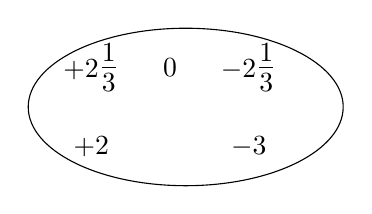
\begin{tikzpicture}
    \draw (2, 0) circle [x radius=2, y radius=1];

    \node at (0.8, 0.5) {$+2${\Large$\frac{1}{3}$}};
    \node at (1.8, 0.5) {$0$};
    \node at (2.8, 0.5) {$-2${\Large$\frac{1}{3}$}};
    \node at (0.8, -0.5) {$+2$};
    \node at (2.8, -0.5) {$-3$};
\end{tikzpicture}

    \caption*{(第 13 题)}
\end{figure}


\xiaoti{一个数的绝对值一定是正数吗? 为什么?}

\xiaoti{有理数中有没有最小的数? 有没有绝对值最小的数?
    有没有最小的正整数? 有没有最小的负整数? 如果有, 各是什么数?
}

\xiaoti{加工一根轴, 图纸上注明它的直径是 $\phi 30\,^{+0.03}_{-0.02}$,
    $\phi 30$ 表示直径是 30 毫米,
    $+0.03$ 表示合格品的直径最大只能比规定直径大 $0.03$ 毫米,
    $-0.02$ 表示合格品的直径最小只能比规定直径小 $0.02$ 毫米。
    那么合格品的直径最大是多少,最小是多少?
}

\begin{figure}[htbp]
    \centering
    \begin{tikzpicture}
    \pgfmathsetmacro{\angle}{45}
    \pgfmathsetmacro{\len}{5}
    \pgfmathsetmacro{\r}{1}

    \coordinate (O) at (0, 0);
    \coordinate (O') at ({\len * cos(\angle)},  {\len * sin(\angle)});
    \coordinate (dA) at ({\r * cos(90 + \angle)}, {\r * sin(90 + \angle)});
    \coordinate (dB) at ({\r * cos(270 + \angle)}, {\r * sin(270 + \angle)});

    \draw (O) circle (\r);
    \draw [pattern={mylines[angle=45, distance={4pt}]}]
        ($(O) + (dA)$) -- ($(O') + (dA)$)
        arc [start angle=90 + \angle, end angle=-90 + \angle, radius=\r]
        -- ($(O) + (dB)$)
        arc [start angle=-90 + \angle, end angle=90 + \angle, radius=\r];

    \draw (-1.5*\r, 0) -- (-\r, 0)
         (\r, 0) -- (1.5*\r, 0);
    \draw [dashed] (-\r, 0) -- (\r, 0);
    \draw (0, -1.5*\r) -- (0, -\r)
         (0, \r) -- (0, 1.5*\r);
    \draw [dashed] (0, -\r) -- (0, \r);

    \begin{scope}[xshift=15em, >=Stealth]
        \draw (0, 0) circle (\r);
        \draw (-1.5*\r, 0) -- (-\r, 0)
             (\r, 0) -- (1.5*\r, 0);
        \draw [dashed] (-\r, 0) -- (\r, 0);
        \draw (0, -1.5*\r) -- (0, -\r)
            (0, \r) -- (0, 1.5*\r);
        \draw [dashed] (0, -\r) -- (0, \r);

        \coordinate (X) at ({\r * cos(\angle)}, {\r * sin(\angle)});
        \coordinate (O) at (0, 0);
        \draw [<->] (X) -- ($(X)!2!(O)$);
        \draw (X) -- ($(X)!-1.5!(O)$) -- +(2, 0)
            node [pos=0.5, above] {$\phi 30\,^{+0.03}_{-0.02}$};
    \end{scope}
\end{tikzpicture}

    \caption*{(第 16 题)}
\end{figure}



\xiaoti{场上 30 袋稻谷过秤, 各袋的千克数记录如下:\\
    \begin{tblr}{columns={3em, $$}, colsep = 0pt, rowsep=0pt}
        93,  &   88,  &   91,  &   90,  &   89,  &   95,  &   86,  &   90,  &   90,  &   86,  \\
        94,  &   87,  &   85,  &   96,  &   94,  &   91,  &   95,  &   84,  &   87,  &   95,  \\
        90,  &   96,  &   89,  &   94,  &   88,  &   93,  &   92,  &   96,  &   90,  &   94\juhao
    \end{tblr} \\
    以每袋 90 千克为准, 超过的千克数记作正数, 不足的千克数记作负数,
    计算超过或不足的总数,并求 30 袋稻谷的总重量。
}


\xiaoti{第三中学男子排球队共有十名队员, 身高分别为:\\
    1.73 米, 1.74 米, 1.70 米, 1.76 米, 1.80 米, \\
    1.75 米, 1.77 米, 1.79 米, 1.74 米, 1.72 米。 \\
    计算男排队员平均身高。
}

\xiaoti{$9$ 与 $-13$ 的和是多少? 它们的和的绝对值是多少? 它们的绝对值的和是多少? 比较三个结果的大小。}

\xiaoti{写出下列各数的相反数和倒数:\jiange \\
    \begin{tblr}{hlines, vlines,
        columns={3em, c, $$},
        column{1} = {mode=text},
    }
        原数 & 5 & -6 & \dfrac{2}{3} & 1 & -0.5 & -1 \\
        相反数 & \\
        倒数 & \\
    \end{tblr} \jiange
}

\xiaoti{任意写出两个互为相反数的数。它们的和与商各是什么?}

\xiaoti{}%
\begin{xiaoxiaotis}%
    \xxt[\xxtsep]{两个有理数相乘, 在什么情况下积是正数? 是负数?是零?}

    \xxt{两个有理相除, 在什么情况下商是1 ? 是 $-1$ ? 是零?没有意义?}

\end{xiaoxiaotis}

\xiaoti{某冷冻厂 \, 一号 \, 库房的室温是 $-2$ ℃, 现有一批食品需要在 $-23$ ℃ 冷藏。
    如果每小时能降温 $4$℃,几小时后就能降到所要求的温度?
}

\xiaoti{煤矿 \, 井下 $A$ 点的标高是 $-174.8$ 米,己知从 $A$ 到 $B$,
    水平距离为 $120$ 米, 每经过水平距离 $10$ 米上升 $0.4$ 米, 求 $B$ 点的标高。
}

\begin{figure}[htbp]
    \centering
    \begin{tikzpicture}[>=Stealth, scale=0.85]
    \clip (0.05, 0) rectangle (7.95, -5.95);
    \draw (0, 0) -- (8, 0);
    \fill [pattern = dots] (0, 0) rectangle (8, -6);

    \filldraw [fill=white] (2, -4.2) -- (6, -3.0) --  (6, -3.8) -- (2, -5.0) -- cycle;

    \filldraw [fill=white] (1.5, 0) rectangle (2.3, -6);
    \filldraw [fill=white] (5.8, 0) rectangle (6.6, -6);

    \fill [fill=white] (2, -4.2) -- (6, -3.0) --  (6, -3.8) -- (2, -5.0) -- cycle;

    \node at (2.0, -4.8) {$A$};
    \node at (6.1, -3.8) {$B$};
    \draw [dashed] (2.3, -4.95) -- (5.8, -4.95)
        node [pos=0.6, below, fill=white, inner sep=3pt] {$120$};
\end{tikzpicture}

    \caption*{(第 24 题)}
\end{figure}


\xiaoti{计算:}
\begin{xiaoxiaotis}

    \begin{tblr}{columns={18em, colsep=0pt}}
        \xxt{$5 \div 0.1$;}        & \xxt{$5 \div 0.01$;} \\
        \xxt{$5 \div 0.001$;}      & \xxt{$5 \div (-0.1)$;} \\
        \xxt{$5 \div (-0.01)$;}    & \xxt{$5 \div (-0.001)$;} \\
        \xxt{$0.2 \div 0.1$;}      & \xxt{$0.02 \div 0.01$;} \\
        \xxt{$0.002 \div 0.001$;}  & \xxt{$(-0.3) \div 0.1$;} \\
        \xxt{$(-0.03) \div 0.01$;} & \xxt{$(-0.003) \div 0.001$。} \\
    \end{tblr}

\end{xiaoxiaotis}


\xiaoti{在下列各式的括号里填上适当的数:}
\begin{xiaoxiaotis}

    \xxt{\begin{tblr}[t]{columns={$}}
        (+5) + (\quad) = +3, \\
        (+5) + (\quad) = -3, \\
        (-5) + (\quad) = +3, \\
        (-5) + (\quad) = -3; \\
    \end{tblr}}

    \xxt{\begin{tblr}[t]{columns={$}}
        (+3) \times (\quad) = -6, \\
        (-3) \times (\quad) = -6, \\
        (+6) \times (\quad) = +3, \\
        (+6) \times (\quad) = -3; \\
    \end{tblr}}

    \xxt{\begin{tblr}[t]{columns={$}}
        (-3) + (\quad) = 0, \\
        (-5) \times (\quad) = 0\juhao \\
    \end{tblr}}

\end{xiaoxiaotis}


\xiaoti{在下面各式的括号里,能不能填上适当的数?}
\begin{xiaoxiaotis}

    \twoInLineXxt[18em]{$0 \times (\quad) = 5$;}{$0 \times (\quad) = 0$。}

\end{xiaoxiaotis}


\xiaoti{平方得 $4$ 的有理数有哪几个? 有没有平方得 $-4$ 的有理数?
        立方得 $8$ 的有理数有哪几个? 有没有立方得 $-8$ 的有理数?
}


\begin{enhancedline}
\xiaoti{计算}
\begin{xiaoxiaotis}

    \xxt{$\left(1\dfrac{3}{4} - \dfrac{7}{8} - \dfrac{7}{12}\right) \times \left(-1\dfrac{1}{7}\right)$;}

    \xxt{$(-81) \div 2\dfrac{1}{4} + \dfrac{4}{9} \div (-16)$;}

    \xxt{$\dfrac{2}{5} \div \left(-2\dfrac{2}{5}\right) - \dfrac{8}{21} \times \left(-1\dfrac{3}{4}\right) - 0.25$;}

    \xxt{$3 (-2.5) (-4) + 5 (-6) (-3)^2$;}

    \xxt{$\{0.85 - [12 + 4 \times (3 - 10)]\} \div 5$;}

    \xxt{$2^2 + (-2)^3 \times 5 - (-0.28) \div (-2)^2$;}

    \xxt{$[(-3)^3 - (-5)^3] \div [(-3) - (-5)]$。}

\end{xiaoxiaotis}
\end{enhancedline}

\xiaoti{按下列程序进行计算,并把各次结果填入表内(如第一次 $(+3) \times (+3) - (-5)$ 得 $14$,不大于 $200$;
    第二次再做,$14 \times (+3) - (-5)$,等等):
}

\begin{minipage}{7cm}
    \centering
    \begin{tikzpicture}[
    >=Stealth,
    skip loop/.style={to path={-- ++(#1, 0) |- (\tikztotarget)}},
]
    \graph [grow down sep = 2em,
        nodes={draw, rectangle, minimum width=7em},
        decision/.style={draw, diamond, aspect=4, inner sep=1pt},
    ]{
        add/"$+3$" [label=above:{输入}] ->
        times/"$\times (+3)$" ->
        sub/"$- (-5)$" ->
        decide/"$>200$" [decision, label=3:{否}] ->["是"]
        stop/"停" [label=below:{输出}];
    };

    \graph[no placement] {
        p1 [coordinate, below=3mm of add];
        (decide.east) -> [skip loop=10mm] (p1);
    };
\end{tikzpicture}

\end{minipage}
\begin{minipage}{7cm}
    \begin{tblr}{hlines, vlines,
        colspec={Q[c,6em]Q[c,6em]},
    }
        计算次数 & 计算结果 \\
        1       & 14       \\
        2       &          \\
        3       &          \\
        4       &          \\
    \end{tblr}
\end{minipage}



\xiaoti{按下列程序进行计算,并把各次结果填入表内:}

\begin{minipage}{7cm}
    \centering
    \begin{tikzpicture}[
    >=Stealth,
    skip loop/.style={to path={-- ++(#1, 0) |- (\tikztotarget)}},
]
    \graph [grow down sep = 2em,
        nodes={draw, rectangle, minimum width=7em},
        decision/.style={draw, diamond, aspect=4, inner sep=1pt},
    ]{
        sub/"$-2$" [label=above:{输入}] ->
        add/"$+ (-1.5)$" ->
        div/"$\div (+2)$" ->
        decide/"$> -1.6$" [decision, label=3:{否}] ->["是"]
        stop/"停" [label=below:{输出}];
    };

    \graph[no placement] {
        p1 [coordinate, below=3mm of sub];
        (decide.east) -> [skip loop=10mm] (p1);
    };
\end{tikzpicture}

\end{minipage}
\begin{minipage}{7cm}
    \begin{tblr}{hlines, vlines,
        colspec={Q[c,6em]Q[c,6em]},
    }
        计算次数 & 计算结果 \\
        1       &          \\
        2       &          \\
        3       &          \\
    \end{tblr}
\end{minipage}

\end{xiaotis}



